\documentclass[11pt]{article}
\usepackage[a4paper,margin=24mm]{geometry}
\usepackage{amsmath,amssymb,mathtools,amsthm,mathrsfs,tikz,pgfplots,longtable,booktabs,array,calc,enumitem}
\usepackage[hidelinks,hypertexnames=false]{hyperref}\usepackage{xurl}
\usepackage{fontspec}\setmainfont{DejaVu Serif}
\usetikzlibrary{arrows.meta,positioning,calc}\pgfplotsset{compat=1.18}
\setlength{\emergencystretch}{4em}\providecommand{\tightlist}{}\newcounter{none}
\setcounter{secnumdepth}{0}\allowdisplaybreaks
\title{The original projection-angle spectrum\\and arithmetic word}
\author{Split-Zero research programme}
\date{21 September 2026\\SZ-20260921-019}
\begin{document}\maketitle
Every original projection direction now has an explicit inverse-growth
bound, with the entire lower-root constraint retained. The complete
long arithmetic word has a controlled spectrum, rectangle resultant,
and observed heat return. The original-root and weighted-source
innovation formulas are joined by an exact vector identity, including
the physical complex phase and source mass.

The centered projection-angle spectrum has a further direction law:
over the entire cutoff window its total downward movement is
$O_{h,A}(\log(q+2)/k)$, tending to zero. The same result holds for
both original Gamma source orders. This sharpens a bounded path
variation to its endpoint increase. Its proof follows the actual
positive source increments, with no discarded low directions.

The native determinant coefficient at order $kq$ remains the
period-dependent endpoint statistic given in AD12--14 and RX17--19.
It has not been assigned a value. The negative intermediate observed
heat return is retained at its exact scope; it does not assign the
separate complex-current signs. Every finite guard, inherited source
status and auxiliary example is identified below.
\begingroup\small\tableofcontents\endgroup\clearpage
\section*{The full projection and its two increments}
\addcontentsline{toc}{section}{The full projection and its two increments}
In the original orthonormal Gamma frame, $E_N$ evaluates every lower
root and $W_N$ contains every original invariant functional. Adding
one degree gives the exact diagram
\[
\begin{array}{ccc}
\ker E_N&\lhook\joinrel\longrightarrow&\ker[E_N,e_N]
=\ker E_N\oplus\mathbb Ct_N\\
\downarrow W_N&&\downarrow[W_N,w_N]\\
\mathbb C^r&=&\mathbb C^r.
\end{array}
\]
The new unit vector and its actual observed image are
\[
t_N=\frac1{\sqrt{\kappa_N}}
\binom{-E_N^*(E_NE_N^*)^{-1}e_N}{1},\qquad
a_N=[W_N,w_N]t_N,
\]
\[
C_{N+1}=C_N+a_Na_N^*,\qquad
B_{N+1}=B_N+w_Nw_N^*.
\]
The first increment retains the full lower-root projection. The second
uses the unrestricted source. RX7--8 proves the exact relation of $a_N$
to the weighted monic source innovation. AD4 then separates their two
effects on every ordered squared angle:
\[
\begin{aligned}
\sum_j(\log s_{j,N}-\log s_{j,N+1})_+
&\le\log\frac{\det B_{N+1}}{\det B_N},\\
\sum_j(\log s_{j,N+1}-\log s_{j,N})_+
&\le\log\frac{\det C_{N+1}}{\det C_N}.
\end{aligned}
\]
The complete first allowance telescopes to $O(q\log q)$, while the
arithmetic determinant scale is $rq\asymp kq$. This is the mechanism
behind the direction law. It bounds all downward steps together.

\begin{figure}[ht]\centering
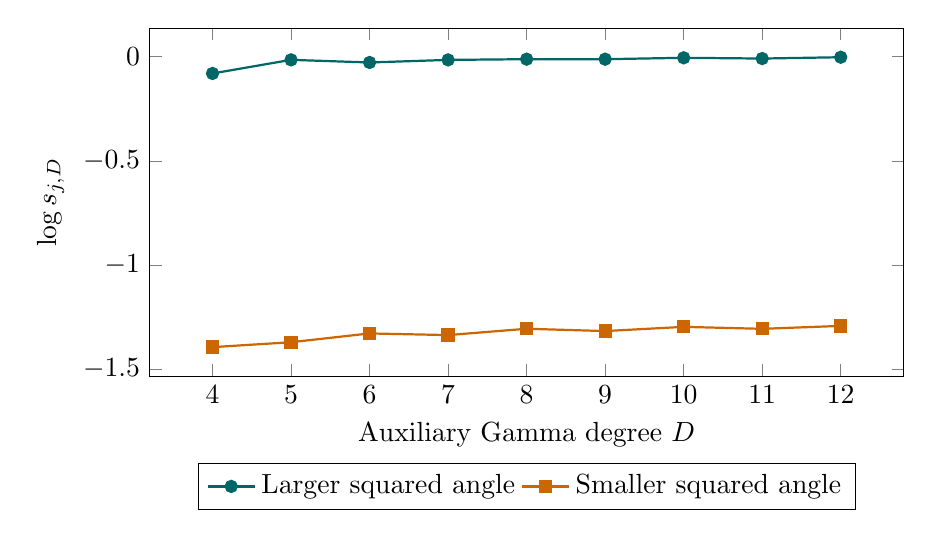
\begin{tikzpicture}\begin{axis}[width=.92\textwidth,height=6cm,
xlabel={Auxiliary Gamma degree $D$},ylabel={$\log s_{j,D}$},
legend style={at={(.5,-.25)},anchor=north,legend columns=2}]
\addplot[teal!80!black,thick,mark=*]coordinates{(4,-0.0804853358718987754940650748581413553565742864587445705896602) (5,-0.0151161498272819476716520376988623046832976914189744657875865) (6,-0.0277583433032593936380759250780130732899667565315568860761151) (7,-0.0153935069137078157368912362792055573624748159734321062818827) (8,-0.0119152094644119890008117664038344240852476751839619254766414) (9,-0.0119576860907335596638342310720556102286966540268289610993177) (10,-0.00533271290946332500687061184278253083151447675480145052017125) (11,-0.00888487246711130408176776483600722393334340561962082615374149) (12,-0.0025130227422906212005521999921368808397359464329059828664081)};
\addlegendentry{Larger squared angle}
\addplot[orange!80!black,thick,mark=square*]coordinates{(4,-1.3941082449079447088139673055618291510171535209963080920957) (5,-1.37046592230097865772022440268515134004252999794394312561811) (6,-1.32835898025955230524839126895135483208275992705757897566933) (7,-1.3362185381567441339853005711105163152410435381041187328047) (8,-1.30586478572492662633985845379600107031536742096897282411777) (9,-1.31696309145376684211592250965719384840178284501946283536343) (10,-1.29670401399123141518535419591071474208228825081389211925895) (11,-1.30618670468624956378864378613660578619555937026304787230502) (12,-1.29213648468155982823059108262649433025794776952566949077723)};
\addlegendentry{Smaller squared angle}
\end{axis}\end{tikzpicture}
\caption{A finite check with the complete lower-root set $\{i,-i\}$
and observation evaluations at $3+2i$ and $-2+i$, in the original
Gamma polynomial convention. Every plotted value comes from the full
projector. Individual angles can move in both directions. The
downward allowance is their complete unprojected Gram increase
(AD4--8). This is an auxiliary example, not native period data.}
\end{figure}\clearpage
\section*{The rectangle profile of the entire word}
\addcontentsline{toc}{section}{The rectangle profile of the entire word}
The literal pivot-interior polynomial $D$ has $q'=(k-7)^2$ roots.
The word $D(M)$ vanishes on that entire primary subspace and has
$\Delta=16k-48$ positive singular directions. Their values retain
the complete cross-resultant between the interior and boundary roots.
FW11--22 evaluates it through the original rectangle potential,
with all lattice, displacement and phase corrections.

\begin{figure}[ht]\centering
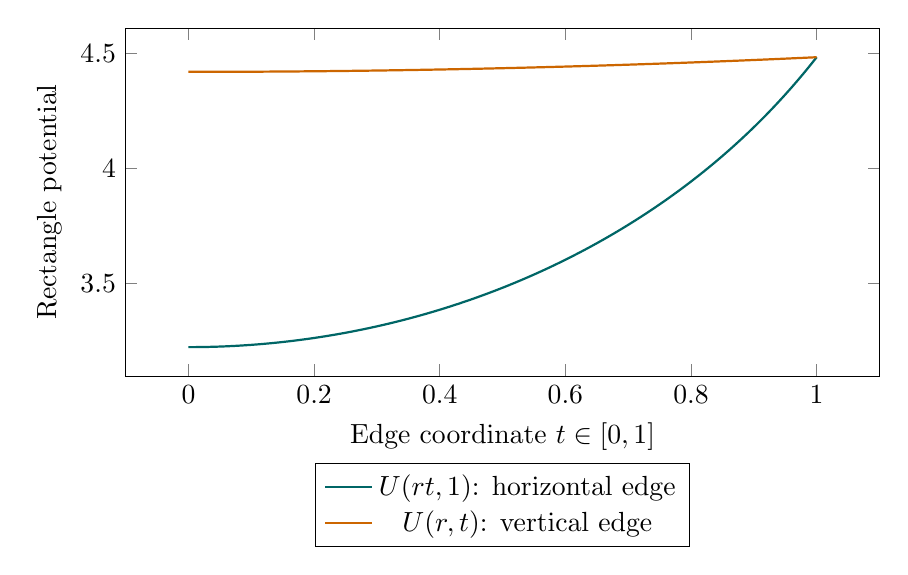
\begin{tikzpicture}\begin{axis}[width=.92\textwidth,height=6cm,
xlabel={Edge coordinate $t\in[0,1]$},ylabel={Rectangle potential},
legend style={at={(.5,-.25)},anchor=north,legend columns=1}]
\addplot[teal!80!black,thick]coordinates{(0.0,3.22237894648192) (0.01,3.22247803726622) (0.02,3.22277532855614) (0.03,3.22327087718364) (0.04,3.22396477793847) (0.05,3.22485716367308) (0.06,3.22594820544984) (0.07,3.22723811273109) (0.08,3.22872713361234) (0.09,3.23041555509944) (0.1,3.23230370343033) (0.11,3.23439194444227) (0.12,3.23668068398563) (0.13,3.23917036838521) (0.14,3.24186148495058) (0.15,3.24475456253661) (0.16,3.24785017215604) (0.17,3.2511489276455) (0.18,3.25465148638721) (0.19,3.25835855008816) (0.2,3.26227086561921) (0.21,3.26638922591653) (0.22,3.27071447094803) (0.23,3.27524748874779) (0.24,3.27998921652149) (0.25,3.28494064182647) (0.26,3.29010280382991) (0.27,3.29547679464935) (0.28,3.30106376077968) (0.29,3.30686490461145) (0.3,3.31288148604547) (0.31,3.31911482420924) (0.32,3.32556629928108) (0.33,3.33223735442838) (0.34,3.33912949786693) (0.35,3.3462443050488) (0.36,3.35358342098682) (0.37,3.36114856272459) (0.38,3.36894152196138) (0.39,3.37696416784231) (0.4,3.38521844992497) (0.41,3.39370640133465) (0.42,3.40243014212124) (0.43,3.41139188283225) (0.44,3.42059392831732) (0.45,3.43003868178133) (0.46,3.43972864910431) (0.47,3.44966644344832) (0.48,3.45985479017307) (0.49,3.47029653208411) (0.5,3.48099463503947) (0.51,3.49195219394329) (0.52,3.50317243915713) (0.53,3.51465874336309) (0.54,3.52641462891541) (0.55,3.53844377572134) (0.56,3.55075002969525) (0.57,3.56333741183467) (0.58,3.57621012797105) (0.59,3.58937257925355) (0.6,3.60282937342917) (0.61,3.61658533698884) (0.62,3.63064552825546) (0.63,3.64501525149696) (0.64,3.65970007215497) (0.65,3.67470583328797) (0.66,3.69003867333628) (0.67,3.70570504532545) (0.68,3.72171173763409) (0.69,3.7380658964616) (0.7,3.75477505014108) (0.71,3.77184713545175) (0.72,3.78929052609313) (0.73,3.80711406349019) (0.74,3.82532709010231) (0.75,3.84393948540902) (0.76,3.86296170474005) (0.77,3.88240482110377) (0.78,3.90228057014404) (0.79,3.92260139831733) (0.8,3.94338051432415) (0.81,3.96463194374733) (0.82,3.98637058673571) (0.83,4.00861227841936) (0.84,4.03137385154118) (0.85,4.05467320053167) (0.86,4.07852934592979) (0.87,4.10296249765743) (0.88,4.12799411518756) (0.89,4.15364696211418) (0.9,4.17994515205791) (0.91,4.20691418226514) (0.92,4.23458095074508) (0.93,4.26297375243002) (0.94,4.29212224975425) (0.95,4.32205741335446) (0.96,4.35281142941856) (0.97,4.38441757162642) (0.98,4.41691003762901) (0.99,4.45032375247965) (1.0,4.48469414411063)};
\addlegendentry{$U(rt,1)$: horizontal edge}
\addplot[orange!80!black,thick]coordinates{(0.0,4.42097890436157) (0.01,4.42098527583552) (0.02,4.42100439025744) (0.03,4.42103624762751) (0.04,4.42108084794603) (0.05,4.42113819121341) (0.06,4.42120827743021) (0.07,4.42129110659708) (0.08,4.42138667871479) (0.09,4.42149499378426) (0.1,4.4216160518065) (0.11,4.42174985278266) (0.12,4.42189639671399) (0.13,4.42205568360188) (0.14,4.42222771344783) (0.15,4.42241248625346) (0.16,4.42261000202052) (0.17,4.42282026075086) (0.18,4.42304326244646) (0.19,4.42327900710944) (0.2,4.42352749474201) (0.21,4.42378872534652) (0.22,4.42406269892542) (0.23,4.4243494154813) (0.24,4.42464887501687) (0.25,4.42496107753494) (0.26,4.42528602303846) (0.27,4.42562371153049) (0.28,4.42597414301422) (0.29,4.42633731749295) (0.3,4.4267132349701) (0.31,4.42710189544921) (0.32,4.42750329893395) (0.33,4.4279174454281) (0.34,4.42834433493557) (0.35,4.42878396746037) (0.36,4.42923634300665) (0.37,4.42970146157868) (0.38,4.43017932318084) (0.39,4.43066992781763) (0.4,4.43117327549367) (0.41,4.43168936621371) (0.42,4.43221819998261) (0.43,4.43275977680536) (0.44,4.43331409668705) (0.45,4.43388115963291) (0.46,4.43446096564828) (0.47,4.43505351473863) (0.48,4.43565880690954) (0.49,4.4362768421667) (0.5,4.43690762051595) (0.51,4.43755114196323) (0.52,4.43820740651459) (0.53,4.43887641417622) (0.54,4.43955816495442) (0.55,4.44025265885561) (0.56,4.44095989588633) (0.57,4.44167987605325) (0.58,4.44241259936315) (0.59,4.44315806582292) (0.6,4.44391627543958) (0.61,4.44468722822028) (0.62,4.44547092417227) (0.63,4.44626736330294) (0.64,4.44707654561979) (0.65,4.44789847113042) (0.66,4.44873313984258) (0.67,4.44958055176414) (0.68,4.45044070690306) (0.69,4.45131360526744) (0.7,4.4521992468655) (0.71,4.45309763170557) (0.72,4.45400875979612) (0.73,4.45493263114571) (0.74,4.45586924576305) (0.75,4.45681860365694) (0.76,4.45778070483632) (0.77,4.45875554931024) (0.78,4.45974313708788) (0.79,4.46074346817852) (0.8,4.46175654259159) (0.81,4.4627823603366) (0.82,4.46382092142321) (0.83,4.46487222586119) (0.84,4.46593627366043) (0.85,4.46701306483094) (0.86,4.46810259938283) (0.87,4.46920487732637) (0.88,4.47031989867191) (0.89,4.47144766342994) (0.9,4.47258817161107) (0.91,4.47374142322602) (0.92,4.47490741828562) (0.93,4.47608615680085) (0.94,4.47727763878278) (0.95,4.47848186424261) (0.96,4.47969883319166) (0.97,4.48092854564138) (0.98,4.4821710016033) (0.99,4.48342620108912) (1.0,4.48469414411063)};
\addlegendentry{$U(r,t)$: vertical edge}
\end{axis}\end{tikzpicture}
\caption{The exact FW rectangle formulas sampled at $r=\gamma/\delta=12$.
Here $U(u,v)=(4r)^{-1}\int_{-r}^r\int_{-1}^1
\log((u-s)^2+(v-t)^2)\,dt\,ds$. The two edge profiles meet at the
corner. FW23--33 proves their pushforward relation to the full
scaled logarithmic spectrum; this parameter illustration makes
no assertion about a native zeta quartet.}
\end{figure}
The full original observed action also retains the collision kernel.
Its intermediate heat return is
\[
\mathcal R\operatorname{Tr}Y_N=-2\Delta+
\operatorname{Tr}\Gamma_{q-1}+\operatorname{Tr}\Gamma_q+o(1),
\qquad0<\Gamma_N\preceq I_{8k-16}.
\]
FW39--49 proves this through the original quotient map, including
the finite $d<m$ correction and the later relative determinant.
The complete human and programme citations occur at the point of
use in each proof and in the accompanying source ledger.
\clearpage

\clearpage\part{Every original projection-angle direction}
\section{Every original projection-angle direction}\label{every-original-projection-angle-direction}

Independent derivation, 21 September 2026. The supplied arrival is checked below with its actual coefficient rows, source measures, physical coordinates and full lower-root projection. The arithmetic endpoint statistic at order kq is not assigned a value. The statements do not close the Riemann hypothesis.

\subsection{AS1. Original objects and finite domain}\label{as1.-original-objects-and-finite-domain}

Fix the original simple quartet, conductor and period. Let \[
\begin{gathered}k\equiv1\pmod4,\quad k\ge17,\quad q=(k+1)^2,\\
k'=k-8,\quad q'=(k-7)^2,\quad 0<\delta<1/2,\quad\gamma>2,
\quad R_h=\sqrt{\delta^2+\gamma^2}.\end{gathered}
\] The estimates using the interval {[}q,2q{]} require the explicit guard \(q\ge2kR_h\). Everything holds eventually for fixed original data. The original exponents and centers are \[
c=k/2,\quad c'=k/2-4,\quad
\beta_{ab}=c+(2a-k)\delta+i(2b-k)\gamma,
\quad\omega_{ab}=(\beta_{ab}-c)/i,
\] \[
\beta'_{ab}=c'+(2a-k')\delta+i(2b-k')\gamma,
\quad\omega'_{ab}=(\beta'_{ab}-c')/i.
\] Thus \(\omega_{ab}=(2b-k)\gamma-i(2a-k)\delta\), and the same formula with k' gives every lower root. Put \[
E_A(w)=\sum_{r,s=0}^8a_{rs}e^{b_{rs}w},\quad
b_{rs}=4+(2r-8)\delta+i(2s-8)\gamma,
\quad A_1=\sum|a_{rs}|,
\] \[
v=\operatorname{ord}_0E_A\le80,\quad
\mu_v=E_A^{(v)}(0)\ne0,\quad d_A=|\mu_v|/v!,\quad
B_A=\max_{a_{rs}\ne0}|b_{rs}|.
\] The bound v≤80 follows because the at most 81 distinct exponents have invertible Vandermonde moment matrix: 81 vanishing initial moments force all coefficients to be zero. The actual conductor is nonzero.

The original invariant rows after the entire low-polynomial constraint form a fixed space \(V_k\), with full row frame Z and coefficient form \[
R_Z=ZZ^*>0,\quad r=r_k=8k-32-v+s_k,\quad
s_k=\dim(K_k\cap\mathcal P_{<v}),\quad0\le s_k\le v.
\] They are supported on the actual conductor strip, whose cardinality is \(n_E=q-q'=16k-48\). At k≥17 one has r≥24, while r≤8k−32. The particular row frame is never replaced by arbitrary exponential rows. Coordinate comparison with \(R_Z\) is a congruence on that same space. The measure is unchanged.

For each original row z put \[
F_z(w)=\sum_\alpha z_\alpha e^{\beta_\alpha w},\quad
G_z(w)=F_z(w)/E_A(w),\quad A_z(w)=e^{-c'w}G_z(w).
\tag{AS1}
\] All derivatives of \(F_z\) of orders below v vanish at zero, so both quotients are holomorphic there. The exact physical functional is \[
\ell_z[f]=[f(-i\partial_w)A_z(w)]_{w=0}
=[f((\partial_w-c')/i)G_z(w)]_{w=0}.
\tag{AS2}
\] Indeed \(\partial_w^n(e^{-c'w}G)=e^{-c'w}(\partial_w-c')^nG\), by induction, and \(e^{-c'w}=1\) at zero. Both c' and −i remain.

For every integer q−1≤N≤2q put D=N−v and M=D−q'. The full lower ideal in physical coordinates is \[
Q_-(y)=i^{-q'}\chi'(c'+iy)=\prod_{a,b=0}^{k'}(y-\omega'_{ab}),
\qquad I_N=Q_-\mathbb C[y]_{\le M}\subset\mathbb C[y]_{\le D}.
\tag{AS3}
\] Multiplication by \(i^{q'}\) is of modulus one; no norm factor is suppressed. Retain \[
d\sigma(y)=\frac{|\Gamma(1/4+iy/2)|^2}{2\pi}\,dy,
\quad M_\sigma=\sqrt{2\pi},
\quad p_{n+1}=yp_n-n(n-1/2)p_{n-1},
\quad\gamma_n=M_\sigma n!(1/2)_n.
\] The frame \(p_n/\sqrt{\gamma_n}\) is the original orthonormal frame. With \((E_D)_{\alpha n}=p_n(\omega'_\alpha)/\sqrt{\gamma_n}\), full-root Lagrange interpolation gives \(\operatorname{rank}E_D=q'\), since D≥q'−1. A polynomial vanishes at all lower roots precisely when it is divisible by Q\_-. Hence \[
P_N=I-E_D^*(E_DE_D^*)^{-1}E_D
\tag{AS4}
\] is the orthogonal projection onto the complete \(I_N\). This follows also by multiplying the matrix: it is self-adjoint, idempotent, kills \(\operatorname{im}E_D^*\), and is identity on \(\ker E_D\).

Let \(W_N\) be the matrix of all these functionals on the orthonormal frame. Define \[
\begin{gathered}C_N=W_NP_NW_N^*,\quad B_N=W_NW_N^*,\quad
S_N=B_N^{-1/2}C_NB_N^{-1/2},\quad
\\ C_N^\circ=R_Z^{-1/2}C_NR_Z^{-1/2},\quad
B_N^\circ=R_Z^{-1/2}B_NR_Z^{-1/2}.
\end{gathered}\tag{AS5}\] The original map is \(\mathcal P_N=P_NT_N\), where \(T_N=W_N^*B_N^{-1/2}:\mathbb C^r\to\mathcal P'_D\). Then \(T_N^*T_N=I\) and \(\mathcal P_N^*\mathcal P_N=S_N\). Its injectivity will follow quantitatively from AS10 below; in particular \(0<S_N\le I\).

\subsection{AS2. All upper roots improve the projected lower bound}\label{as2.-all-upper-roots-improve-the-projected-lower-bound}

For fixed upper lattice point α, set \(r_{\alpha\beta}=\max(|a_\alpha-a_\beta|,|b_\alpha-b_\beta|)\). The exact rectangular coordinates give \[
|\omega_\alpha-\omega_\beta|^2
=4\gamma^2(b_\alpha-b_\beta)^2+4\delta^2(a_\alpha-a_\beta)^2
\ge4\delta^2r_{\alpha\beta}^2.
\] The shell r=j contains at most 8j lattice points; truncating it at the box boundary can only decrease this count. Because log t≤t−1 for t\textgreater0, \[
\sum_{\beta\ne\alpha}\log(k/r_{\alpha\beta})
\le\sum_{j=1}^k8j\log(k/j)
\le8\sum_{j=1}^k(k-j)=4k(k-1)\le4q.
\] Exponentiating proves, without dropping any root, \[
\prod_{\beta\ne\alpha}|\omega_\alpha-\omega_\beta|
\ge(2\delta k)^{q-1}e^{-4q}.
\tag{AS6}
\]

In the orthonormal Gamma recurrence, multiplication by y has upper and lower shift weights √((n+1)(n+1/2)) and √(n(n−1/2)). Each is at most D+1 on degree≤D. The triangle inequality gives \[
\|(y-z)p\|_\sigma\le[2(D+1)+|z|]\|p\|_\sigma.
\tag{AS7}
\] Apply this successively to all q−1 factors of the Lagrange numerator. Every root has modulus≤\(kR_h\). The squared operator norm of the full interpolation map from root values to polynomials is at most the sum of its q squared column norms, thus at most \[
B_{\mathrm{val},k}=qM_\sigma e^{8q}
\left(\frac{2q+kR_h}{2\delta k}\right)^{2(q-1)}.
\tag{AS8}
\] Consequently every full upper-root row h has Gamma functional norm at least \(B_{\mathrm{val},k}^{-1/2}\|h\|_2\): compose its evaluation row with this exact interpolation right inverse.

We also require a forward bound for the original conductor matrix \(A_{D,1}\). Let \[
\mathfrak M_k=\max\{1,e^{1+2\pi\gamma}A_1
(8q+1)^{1/4}(2q+1)(4q+1)^{4\delta}\}.
\tag{AS9}
\] Here is a direct verification including v. Put \(w(t)=-i\arctan t\) and \(g(t)=t^{-v}e^{-4w(t)}E_A(w(t))\). For m=j+v≥1 choose radius m/(m+1). The right-half-plane logarithm of (1−it)/(1+it) gives \(|e^{(b_{rs}-4)w(t)}|\le e^{2\pi\gamma}(2m+1)^{4\delta}\). Cauchy's coefficient estimate applied to \(t^vg(t)\) gives \(|g_j|\le e^{1+2\pi\gamma}A_1[2(j+v)+1]^{4\delta}\). For m=0, \(g_0=E_A(0)\), and the same inequality holds directly. The exact WCF matrix is \((A_{D,1})_{ij}=g_{j-i}\rho_{j+v}/\rho_i\) for i≤j, with \(\rho_n^2=n!/(1/2)_n\). All \(\rho_i\ge1\). Induction proves \(\rho_n^4\le4n+1\): the needed one-step difference is \((4n+5)(n+1/2)^2-(4n+1)(n+1)^2=1/4\). Thus every nonzero entry is bounded by the product in AS9 without the factor 2q+1. There are at most D+1≤2q+1 entries in each row and column. The inequality \(\|A\|_2^2\le\|A\|_1\|A\|_\infty\), obtained by weighted Cauchy--Schwarz, proves \(\|A_{D,1}\|\le\mathfrak M_k\).

Let \(a_*\) be the actual nonzero lexicographic conductor pivot and \(C_{\mathrm{path}}=A_1/|a_*|\ge1\). Original elimination replaces the pivot \((r_0+i,s_0+j)\) by all other terms \(-a_{rs}/a_*\) at (r+i,s+j). Height 9a+b strictly decreases: when \(r<r_0\) the decrease is at least 9−8=1, and when \(r=r_0\) it is \(s_0-s\ge1\). Heights range from 0 to 10k. A substitution path therefore has length≤10k. The sum of absolute outgoing edge weights is \(C_{\mathrm{path}}-1\), so the sum of terminal-path weights is at most \(\sum_{j=0}^{10k}(C_{\rm path}-1)^j\le C_{\rm path}^{10k}\). Consequently the exact strip map has \(\|N_k\|_2\le\sqrt qC_{\rm path}^{10k}\), \(N_kz=z\) on the strip and \(N_kM_A=0\) on the full conductor image. It follows that \(\operatorname{dist}(z,\operatorname{im}M_A)\ge\|z\|/(\sqrt qC_{\rm path}^{10k})\).

To transfer this distance through the actual projection, for any lower evaluation row \(bE_D\) use the exact duality \(F_z=E_AG_z\). Multiplication by the original \(A_{D,1}\) sends \(W_z-bE_D\) to the full upper Gamma functional row of \(z-M_Ab\), with its first v identically zero entries removed. The equality of exponent coordinates is \(\beta'_{ij}+b_{rs}=\beta_{i+r,j+s}\), so this is the entire original conductor image. The zero entries do not change the norm. AS8, AS9 and the strip-distance estimate give \[
\inf_b\|W_z-bE_D\|^2
\ge c_k\|z\|^2,\qquad
c_k=[\mathfrak M_k^2B_{\mathrm{val},k}qC_{\rm path}^{20k}]^{-1}.
\tag{AS10}
\] The infimum is exactly \(\|W_zP_N\|^2\), by AS4. Hence \(C_N^\circ\succeq c_kI\). This proves injectivity with the full projection retained.

The exact useful logarithmic expansion is \[
\log(1/c_k)=2(q-1)\log(q/k)+8q
+2(q-1)\log\frac{2+kR_h/q}{2\delta}
+2\log\mathfrak M_k+\log(q^2M_\sigma)+20k\log C_{\rm path}.
\tag{AS11}
\] All terms after the first are O(q) for fixed original data. In particular no q log k loss has been inserted in the remainder.

\subsection{AS3. Cancellation of the actual conductor zeros}\label{as3.-cancellation-of-the-actual-conductor-zeros}

To avoid a collision between two meanings of \(b_A\), write \(b(w)=E_A(w)/w^v\), \(a_0=\log^+(A_1/d_A)/\log2\), \(b_0=4B_A/\log2\). The function b is entire and \(|b(0)|=d_A\). For R≥1, Jensen's formula at radius 4R gives \[
n_A(2R)\le a_0+b_0R,
\tag{AS12}
\] where \(n_A\) counts zeros of b in the open disk \textbar w\textbar\textless2R with multiplicity. To see this without a boundary assumption, factor the finitely many interior zeros of b and apply the mean-value identity to the logarithm of the zero-free quotient on radii approaching 4R. Each zero of modulus\textless2R contributes more than log2. On \textbar w\textbar=4R, \(|b(w)|\le A_1(4R)^{-v}e^{4B_AR}\le A_1e^{4B_AR}\). The resulting bound is \((\log(A_1/d_A)+4B_AR)/\log2\); replacing the first logarithm by its positive part proves AS12. Zeros exactly on either count boundary cause no failure of the bound.

Define the actual row subspace \[
\mathcal Z_R=\{z\in V_k:F_z^{(j)}(\zeta)=0
\text{ for every }b(\zeta)=0,\ |\zeta|<2R,\ 0\le j<\operatorname{ord}_\zeta b\}.
\tag{AS13}
\] These are linear value-and-jet equations on the same rows Z. Their rank is their true codimension, which is at most \(n_A\)(2R); independence is unnecessary.

Take the finite radius-2R Blaschke product \(\mathcal B_R(w)=\prod_\zeta [2R(w-\zeta)/((2R)^2-\bar\zeta w)]^{m_\zeta}\). There is no zero at zero because b(0)≠0. Both \(b/\mathcal B_R\) and \(e^{-c'w}F_z(w)/(w^v\mathcal B_R(w))\) extend holomorphically across the canceled zeros; the first has no zero in the open disk. All factor poles lie strictly outside the closed disk, and \(|\mathcal B_R|=1\) on its boundary. Put \(M_R^b=\max(A_1,d_A)e^{2B_AR}\). The maximum principle gives \(|b/\mathcal B_R|\le M_R^b\), and \(|(b/\mathcal B_R)(0)|\ge d_A\). The nonnegative harmonic function \(u=\log(M_R^b/|b/\mathcal B_R|)\) satisfies \(u(w)\le3u(0)\) for \textbar w\textbar≤R. This follows from the Poisson kernel on any intermediate circle, whose maximum is (s+\textbar w\textbar)/(s−\textbar w\textbar), followed by s↑2R. Thus boundary zeros of b do not require cancellation. Rearranging gives \(|b/\mathcal B_R|\ge d_A^3/(M_R^b)^2\).

On \textbar w\textbar=2R, each centered exponent \(\beta_\alpha-c'\) has modulus≤4+\(kR_h\). Since \((2R)^{-v}\le1\) and z is supported on \(n_E\) positions, \[
|e^{-c'w}F_z(w)/w^v|
\le\sqrt{n_E}e^{2(4+kR_h)R}\|z\|.
\] The maximum principle for the numerator divided by \(\mathcal B_R\) and the last denominator bound prove \[
\max_{|w|\le R}|A_z(w)|
\le C_A\sqrt{n_E}e^{(2kR_h+8+4B_A)R}\|z\|,
\quad C_A=\max(A_1,d_A)^2/d_A^3,
\quad z\in\mathcal Z_R.
\tag{AS14}
\]

For uncanceled rows use \(\bar B_A=\max(1,B_A)\) and \[
\rho_A=\min\left\{1,
\frac{(v+1)!d_A}{2A_1\bar B_A^{v+1}e^{\bar B_A}}\right\}.
\tag{AS15}
\] For \textbar w\textbar≤1 the exponential series bounds \[
|b(w)-b(0)|\le
\frac{A_1\bar B_A^{v+1}}{(v+1)!}|w|e^{\bar B_A|w|}.
\] Indeed \((v+1+j)!\ge(v+1)!j!\); sum the remainder series after dividing by \(w^v\). Therefore \(|b|\ge d_A/2\) on this disk. Bound the centered numerator on its boundary and use its removable value at zero. The maximum principle proves \[
\max_{|w|\le\rho_A}|A_z(w)|\le M_{0,k}\|z\|,
\quad M_{0,k}=2\sqrt{n_E}\rho_A^{-v}d_A^{-1}
e^{(4+kR_h)\rho_A}.
\tag{AS16}
\] No first symbol coefficient has been set equal to one.

\subsection{AS4. The full Gamma ideal norm controls every derivative}\label{as4.-the-full-gamma-ideal-norm-controls-every-derivative}

The original Gamma product at a=1/4 and t=y/2 yields \[
\frac{|\Gamma(a+it)|^2}{\Gamma(a)^2}
=\prod_{n\ge0}(1+t^2/(n+a)^2)^{-1}.
\] For the decreasing nonnegative function f(x)=log(1+t²/x²), \(\sum_{n\ge1}f(n+a)\le\int_a^\infty f(x)dx\le\int_0^\infty f(x)dx=\pi|t|\). The integral follows by differentiating in \textbar t\textbar\textgreater0, obtaining π, and taking its zero limit; equivalently integrate by parts after x=\textbar t\textbar u. Keeping the n=0 factor proves \[
\sigma(y)\ge c_\sigma e^{-\pi|y|/2}/(1+4y^2),
\qquad c_\sigma=\Gamma(1/4)^2/(2\pi).
\tag{AS17}
\] Every lower root has modulus≤\(kR_h\)≤q/2. Thus on q≤y≤2q, \(|Q_-(y)|\ge(q/2)^{q'}\), and the full-line norm has the lower bound \[
\|Q_-p\|_\sigma^2\ge
\frac{c_\sigma q e^{-\pi q}}{1+16q^2}(q/2)^{2q'}
\|p(q\,\cdot)\|_{L^2[1,2]}^2.
\tag{AS18}
\] The interval gives an inequality for the original full measure; it does not define a replacement measure.

Here are details of the coefficient estimate. Rodrigues' formula gives the orthonormal polynomials \(\sqrt{2n+1}P_n(2x-3)\) on {[}1,2{]}. Orthogonality implies all their n roots lie in (1,2): otherwise the product of factors at sign-changing roots there, of degree\textless n, has product with the polynomial of one nonzero sign, contrary to orthogonality. The leading coefficient is positive, so the coefficients alternate and their absolute sum is \(\sqrt{2n+1}P_n(5)\). The integral \(P_n(x)=\pi^{-1}\int_0^\pi(x+\sqrt{x^2-1}\cos\theta)^n d\theta\) for x≥1 follows by summing the geometric series inside the integral and obtaining \((1-2xt+t^2)^{-1/2}\), the read original Legendre generating function. Hence \(P_n(5)\le(5+\sqrt{24})^n\le10^n\). If \(p(qx)=\sum d_n\sqrt{2n+1}P_n(2x-3)\), the triangle inequality and Cauchy--Schwarz give \[
\|\operatorname{coef}p(q\,\cdot)\|_1
\le\Big(\sum_{n=0}^M(2n+1)100^n\Big)^{1/2}\|p(q\,\cdot)\|_2
\le(M+1)10^M\|p(q\,\cdot)\|_2.
\] Writing \(M_{\max}=2q-v-q'\), define \[
\mathfrak A_k=(M_{\max}+1)10^{M_{\max}}2^{q'}e^{\pi q/2}
\sqrt{(1+16q^2)/(c_\sigma q)}.
\tag{AS19}
\] Combining with AS18 proves \[
\|\operatorname{coef}p(q\,\cdot)\|_1
\le\mathfrak A_kq^{-q'}\|Q_-p\|_\sigma.
\tag{AS20}
\]

Suppose \(\max_{|w|\le R}|A_z(w)|\le H_R\|z\|\). Cauchy's estimate applied to AS2 gives \(|\ell_z[y^n]|\le H_R\|z\|n!R^{-n}\le H_R\|z\|(D/R)^n\) for n≤D. Put t=D/R. The full coefficient sum of Q\_- is at most \((kR_h+t)^{q'}\). For \(p(y)=\sum p_jy^j\), \(\sum|p_j|t^j\le\max(1,t/q)^M\sum|p_j|q^j\). Multiply the two sums and use AS20 to obtain the exact functional norm bound \[
\|\ell_z|_{I_N}\|\le\mathfrak A_kH_R
\left(kR_h/q+D/(qR)\right)^{q'}
\max(1,D/(qR))^M\|z\|.
\tag{AS21}
\] For 2≤R≤k, the last maximum is one since D≤2q. Also \(kR_hR\le k^2R_h\le qR_h\), so the other parenthesis is at most (\(R_h\)+2)/R. AS14 therefore proves \[
\|\ell_z|_{I_N}\|\le\mathfrak F_kR^{-q'}\|z\|,
\quad\mathfrak F_k=\mathfrak A_kC_A\sqrt{n_E}
e^{2R_hq+(8+4B_A)k}(R_h+2)^{q'},\quad z\in\mathcal Z_R.
\tag{AS22}
\] For all rows, AS16 and AS21 instead give \[
\|\ell_z|_{I_N}\|\le\mathfrak F_{0,k}\|z\|,
\quad\mathfrak F_{0,k}=\mathfrak A_kM_{0,k}
(kR_h/q+2/\rho_A)^{q'}(2/\rho_A)^{M_{\max}}.
\tag{AS23}
\] Here \(\log\mathfrak A_k\), \(\log\mathfrak F_k\) and \(\log\mathfrak F_{0,k}\) are O(q): \(M_{\max}\le2q\), q'≤q and all conductor/quartet factors except k are fixed. All derivatives through D were included.

\subsection{AS5. Every eigenvalue and the actual squared angles}\label{as5.-every-eigenvalue-and-the-actual-squared-angles}

Order the eigenvalues of \(C_N^\circ\) as \(\lambda_{1,N}\ge\cdots\ge\lambda_{r,N}\). Put \[
L_A=b_0+9,\quad
j_A=\left\lceil\max\{2(a_0+1),a_0+1+4L_A\}\right\rceil,
\quad R_j=(j-1-a_0)/(2L_A).
\tag{AS24}
\] For \(j_A\le j\le r\), first \(j-1-a_0\ge4L_A\), so \(R_j\ge2\). Second \(j\ge2(a_0+1)\) gives \(R_j\ge j/(4L_A)\). Third \(R_j<r/(2L_A)\le(8k-32)/18<k\). Finally \[
a_0+b_0R_j
\le a_0+(j-1-a_0)/2=(j-1+a_0)/2<j.
\] Thus the actual cancellation space has codimension at most j−1. In the coefficient-orthonormal row frame, AS22 bounds its covariance quadratic form by \(\mathfrak F_k^2R_j^{-2q'}\). Diagonalizing \(C_N^\circ\) proves the min--max step directly: if \(\lambda _j\) exceeded that number, the span of its first j eigenvectors would intersect this codimension\textless j space nontrivially and violate the quadratic-form bound. Therefore \(\lambda_{j,N}\le\mathfrak F_k^2(4L_A/j)^{2q'}\). For j\textless{}\(j_A\), AS23 suffices. Define \[
\mathfrak U_k=\max\{\mathfrak F_k^2(4L_A)^{2q'},
\mathfrak F_{0,k}^2j_A^{2q'}\}.
\] AS10 gives the full enclosure \[
c_k\le\lambda_{j,N}\le\mathfrak U_kj^{-2q'},
\quad1\le j\le r,\quad\log\mathfrak U_k=O(q).
\tag{AS25}
\] If \(j_A\)\textgreater r, the second term still proves every finite upper bound. No rank or cancellation independence assumption is needed.

The strip interpolation bound, using AS7 on exactly its \(n_E\) nodes with separation≥2δ, is \[
B_E=n_EM_\sigma\left(\frac{2n_E+kR_h}{2\delta}\right)^{2(n_E-1)}.
\] The actual upper functional row is \(W_zA_{D,1}\) and has its first v entries zero. Strip interpolation therefore gives \(\|W_z\|\ge\|z\|/(\mathfrak M_k\sqrt{B_E})\). Thus \[
B_N^\circ\succeq b_k^-I,
\quad b_k^-=(\mathfrak M_k^2B_E)^{-1}.
\tag{AS26}
\] For an upper bound take \(t_A=\tanh(\rho_A/2)\), so \(|\arctan t|\le\sum_{j\ge0}|t|^{2j+1}/(2j+1)
=\operatorname{arctanh}|t|\le\rho_A/2\). The original generating function is \[
H_z(t)=(1+t^2)^{-1/4}A_z(-i\arctan t)=\sum a_{z,n}t^n,
\quad W_{z,n}=\rho_na_{z,n}/\sqrt{M_\sigma}.
\tag{AS27}
\] It follows by applying AS2 to the exact Gamma generating function \(\sum p_n(y)t^n/n!=(1+t^2)^{-1/4}e^{y\arctan t}\). AS16 and Cauchy's coefficient bound give \(|a_{z,n}|\le M_{0,k}(1-t_A^2)^{-1/4}t_A^{-n}\|z\|\). Since \(\rho_n^2\le2n+1\) and \(\sum_{n=0}^D(2n+1)=(D+1)^2\), \[
B_N^\circ\preceq b_k^+I,\qquad
b_k^+=\max\left\{1,
\frac{M_{0,k}^2(1-t_A^2)^{-1/2}}{M_\sigma}
(2q+1)^2t_A^{-4q}\right\}.
\tag{AS28}
\] The bounds are for all row combinations, hence contain no extra factor r.

The explicit unitary \(U_N=B_N^{1/2}R_Z^{-1/2}(B_N^\circ)^{-1/2}\) satisfies \(U_N^*U_N=I\) and \(U_N^*S_NU_N=(B_N^\circ)^{-1/2}C_N^\circ(B_N^\circ)^{-1/2}\). Generalized min--max applied to the Rayleigh quotient \(u^*C_N^\circ u/(u^*B_N^\circ u)\), using AS25--28, proves the actual squared-angle enclosure \[
\frac{c_k}{b_k^+}\le s_{j,N}\le
\min\left\{1,\frac{\mathfrak U_k}{b_k^-}j^{-2q'}\right\},
\qquad s_{1,N}\ge\cdots\ge s_{r,N}>0.
\tag{AS29}
\] Every original lower-root constraint remains in \(C_N\).

\subsection{AS6. A bounded centered spectrum, volume and all inverse exterior ranks}\label{as6.-a-bounded-centered-spectrum-volume-and-all-inverse-exterior-ranks}

Set \(\ell_k=\log(q/k)\), \(x_{j,N}=q^{-1}\log s_{j,N}+2\ell_k\) and \[
C_k^{\mathrm{ang}}=\max\left\{0,
-q^{-1}\log(c_k/b_k^+)-2\ell_k,
q^{-1}\log(\mathfrak U_k/b_k^-)+2\ell_k
-(2q'/q)\log r\right\}.
\tag{AS30}
\] This is a finite explicit number and is O(1). Here are all contributions to that claim. AS11 yields \(q^{-1}\log(1/c_k)-2\ell_k=O(1)\); the difference between q−1 and q contributes exactly \(-2\ell_k/q\). AS28 gives \(q^{-1}\log b_k^+=O(1)\), because \(\rho _A\),\(t_A\) are fixed positive numbers and \(\log M_{0,k}=O(k+\log k)\). Also \(\log(1/b_k^-)=O(k\log(k+2))\), and AS25 gives \(\log\mathfrak U_k=O(q)\). Finally \[
2\ell_k-(2q'/q)\log r
=2\log\frac{q}{kr}+2(1-q'/q)\log r=O(1),
\] since r=8k+O(1), q/k²→1 and 1−q'/q=(16k−48)/q. Thus the centered constant is bounded for fixed original data; this proof never asserts uniformity when \(d_A\) or \textbar{}\(a_*\)\textbar{} tends to zero.

AS29 and q'≤q give \[
-C_k^{\mathrm{ang}}\le x_{j,N}
\le C_k^{\mathrm{ang}}+(2q'/q)\log(r/j)
\le C_k^{\mathrm{ang}}+2\log(r/j).
\tag{AS31}
\] The elementary integral estimate \(\sum_{j=1}^r\log(r/j)\le r\) follows from \(\log(r!)\ge\int_1^r\log t\,dt=r\log r-r+1\). Summation proves the finite determinant enclosure \[
-2rq\ell_k-C_k^{\mathrm{ang}}rq
\le\log\det S_N
\le-2rq\ell_k+(C_k^{\mathrm{ang}}+2)rq.
\tag{AS32}
\] Therefore uniformly on the entire integer cutoff window, \[
\log\det S_N=-2r_kq\log(q/k)+O(kq),\qquad
\frac{\log\det S_N}{kq\log(q/k)}\longrightarrow-16.
\tag{AS33}
\] AS31 also gives \(|x_{j,N}|\le C_k^{\mathrm{ang}}+2\log(r/j)\), and hence the full empirical estimate \[
\frac1r\sum_{j=1}^r
\left|\frac{-\log s_{j,N}}{2q\ell_k}-1\right|
\le\frac{C_k^{\mathrm{ang}}+2}{2\ell_k}.
\tag{AS34}
\]

The inverse of the exact map \(\mathcal P_N=P_NT_N\) is taken only on its image, with the inherited lower Gamma norm. Its singular values are \(s_{r,N}^{-1/2},\ldots,s_{1,N}^{-1/2}\). Thus \[
\log\|\wedge^p\mathcal P_N^{-1}\|
=pq\ell_k-\frac q2\sum_{j=r-p+1}^r x_{j,N}.
\] The average of the last p values of the decreasing sequence log(r/j) is no larger than its full average≤1. AS31 proves simultaneously for every 1≤p≤r that \[
pq\left(\ell_k-\frac{C_k^{\mathrm{ang}}+2}{2}\right)
\le\log\|\wedge^p\mathcal P_N^{-1}\|
\le pq\left(\ell_k+\frac{C_k^{\mathrm{ang}}}{2}\right).
\tag{AS35}
\] Division by pq\(\ell\)\_k gives a uniform limit of one over N and p.

For any actual p-dimensional subspace X of the original row space, restrict both covariances before forming \(S_{X,N}\). AS10 and AS28 give every restricted squared angle≥\(c_k\)/\(b_k\)\^{}+. Restriction of generalized min--max gives its jth squared angle≤the full \(s_{j,N}\). Multiplication of AS29 for j≤p proves \[
p\log(c_k/b_k^+)\le\log\det S_{X,N}
\le\min\{0,p\log(\mathfrak U_k/b_k^-)-2q'\log(p!)\}.
\tag{AS36}
\] No identification of \(S_{X,N}\) with a principal submatrix of \(S_N\) is used.

\subsection{AS7. Exponential tails and full cutoff variation}\label{as7.-exponential-tails-and-full-cutoff-variation}

Write \(C=C_k^{\mathrm{ang}}\). For u≥C, AS31 implies \(x_{j,N}>u\Rightarrow j<r e^{-(u-C)/2}\), and consequently \(\#\{j:x_{j,N}>u\}\le r e^{-(u-C)/2}\). Integrate this count from T to infinity to obtain, for T≥C, \[
\frac1r\sum_j(x_{j,N}-T)_+
\le2e^{-(T-C)/2}.
\tag{AS37}
\] There is no lower tail below −C. For 0≤θ\textless1/2, monotonicity of \(t^{-2\theta}\) gives \(\sum_{j=1}^r j^{-2\theta}\le\int_0^r t^{-2\theta}dt
=r^{1-2\theta}/(1-2\theta)\). Therefore \[
\frac1r\sum_j e^{\theta x_{j,N}}
\le e^{\theta C}/(1-2\theta).
\tag{AS38}
\] These bounds, with C=O(1), prove uniform integrability of the centered logarithms at the kq determinant scale.

The same row functionals act on nested spaces \(I_N\subset I_{N+1}\) and \(\mathcal P'_D\subset\mathcal P'_{D+1}\). Each inclusion adds exactly one unit orthogonal polynomial direction. Parseval therefore gives the exact fixed-row updates \[
C_{N+1}=C_N+a_Na_N^*,\qquad B_{N+1}=B_N+b_Nb_N^*.
\tag{AS39}
\] These are ACC17's full ideal and Gamma columns. Let \(\tau _j\) be the ordered generalized eigenvalues of \((C_{N+1},B_N)\). Min--max gives \(\tau_j\ge s_{j,N}\) and \(\tau_j\ge s_{j,N+1}\). Hence \[\begin{gathered}
\sum_j|\log s_{j,N+1}-\log s_{j,N}|
\\\le\sum_j(\log\tau_j-\log s_{j,N})
+\sum_j(\log\tau_j-\log s_{j,N+1})
\\=\log\frac{\det C_{N+1}}{\det C_N}
+\log\frac{\det B_{N+1}}{\det B_N}.
\end{gathered}\tag{AS40}\] This proves the sorted-spectrum variation bound even when individual squared angles change direction or collide.

For completeness the finite unprojected determinant allowance can be specified from already proved original forward and determinant estimates. Use \[
V_N=\frac{qe^2}{M_\sigma}(N+1)^{3/2}(2N+1)^{kR_h+1},
\quad J_D=(D+1)\log^+(1/d_A),
\] \[
K_N=\max\{r\log^+(\mathfrak M_k^2B_E),
r\log^+V_N+2(D+1)\log\mathfrak M_k+2J_D\}.
\tag{AS41}
\] The root-evaluation bound \(V_N\) follows directly from the generating function before division by \(E_A\). At radius \(r_N=N/(N+1)\), one has \(r_N^{-n}\le e\) for n≤N, \(|\arctan t|\le\tfrac12\log(2N+1)\), and \(|1+t^2|^{-1/2}\le(N+1)/\sqrt{2N+1}\). Squaring Cauchy's coefficient bound and multiplying by \(\rho_n^2/M_\sigma\) gives \[
|\phi_n(\omega_\alpha)|^2\le\frac{e^2}{M_\sigma}
\frac{\sqrt{4N+1}(N+1)}{\sqrt{2N+1}}(2N+1)^{kR_h}.
\] The prefactor without \(e^2/M_\sigma\) is at most \((N+1)^{1/2}(2N+1)\), since \((4N+1)(N+1)\le(2N+1)^3\); their difference is \(8N^3+8N^2+N\ge0\). Sum over N+1 degrees and q original roots to obtain the stated \(V_N\). This is the CGR10/KF33 constant. The triangular matrix has \(|\det A_{D,1}|=d_A^{D+1}\prod_{i=0}^D\rho_{i+v}/\rho_i\ge d_A^{D+1}\). The singular-value complement identity gives \(\|\wedge^j A_{D,1}^{-1}\|\le\mathfrak M_k^{D+1-j}e^{J_D}\). Apply this to \(W_N=B_FA^{-1}\) and \(B_FB_F^*\preceq V_NR_Z\); together with AS26 it proves \[
|\log(\det B_N/\det R_Z)|\le K_N=O(q\log(q+2)).
\tag{AS42}
\] The slightly larger common \(\mathfrak M_k\) leaves CGS17's order unchanged and makes every constant here explicit.

Let \(\mu_{k,N}=r^{-1}\sum_j\delta_{x_{j,N}}\). For ordered empirical measures on the real line the optimal \(W_1\) matching is the ordered one: any crossed pairing a≤b,c≤d satisfies \textbar a−c\textbar+\textbar b−d\textbar≤\textbar a−d\textbar+\textbar b−c\textbar, and successively removing crossings proves the claim. Thus \(W_1\) is \(r^{-1}\) times the sum of ordered absolute differences. Sum AS40 over N=q−1,\ldots,2q−1 and telescope both determinants. Since det C=det S det B, AS32 gives \[
\sum_{N=q-1}^{2q-1}W_1(\mu_{k,N+1},\mu_{k,N})
\le2C_k^{\mathrm{ang}}+2+
\frac{2(K_{q-1}+K_{2q})}{rq}.
\tag{AS43}
\] The last term tends to zero. This is a bound on the complete path, not a deduction from endpoint weak convergence.

\subsection{AS8. Both original Gamma source orders}\label{as8.-both-original-gamma-source-orders}

Write \(k=4\ell+1\). The original order-s source is \[
dm_s(y)=\frac{(2\pi)^{s/2}2^{s/2}}{4\pi\Gamma(s/2)}
|\Gamma(s/4+iy/2)|^2dy,\qquad s\in\{1,k\}.
\] For s=1 this equals dσ. Applying Γ(z+1)=zΓ(z) exactly \(\ell\) times, without rescaling the source mass, gives \[
dm_k(y)=\beta_k\prod_{j=0}^{\ell-1}[y^2+(2j+1/2)^2]d\sigma(y),
\qquad\beta_k=(2\pi)^{k/2}/(\sqrt2\Gamma(k/2)).
\tag{AS44}
\] For any P of degree≤D, each positive factor is at least (2j+1/2)², proving the lower comparison. For the upper comparison, write the product as the squared modulus of \(\prod_j(y+i(2j+1/2))\), and apply AS7 successively. Before the jth multiplication the degree is at most D+j. Hence \[
a_{k,D}\|P\|_\sigma^2\le\|P\|_{m_k}^2\le b_{k,D}\|P\|_\sigma^2,
\] \[
a_{k,D}=\beta_k\prod_{j<\ell}(2j+1/2)^2,
\quad b_{k,D}=\beta_k\prod_{j<\ell}[2(D+j+1)+2j+1/2]^2.
\tag{AS45}
\] This full-line comparison is valid on the entire source and on \(I_N\), with unchanged lower roots and center. For the norm of a fixed functional, taking the supremum \(|\ell(P)|^2/\|P\|^2\) reverses these inequalities. Thus both restricted and unrestricted covariances have comparisons \(b^{-1}C^{(1)}\preceq C^{(k)}\preceq a^{-1}C^{(1)}\), and likewise for B. Their generalized Rayleigh quotients are within factors a/b and b/a. Generalized min--max proves, for every j, \[
|\log s_{j,N}^{(k)}-\log s_{j,N}^{(1)}|
\le L_{k,D}:=\log(b_{k,D}/a_{k,D})
=2\sum_{j<\ell}\log\frac{2(D+j+1)+2j+1/2}{2j+1/2}.
\tag{AS46}
\] This sum is O(k log(q+2)), uniformly D≤2q. A finite common bound is \(L_k^{\max}=2\ell\log(8q+8\ell+5)\), since the denominator≥1/2. The source mass \(\beta _k\) cancels only in the displayed angle ratio, after both physical metrics have been retained.

For the original four signs \(\mathcal Rf=f_{q-1}+f_q-f_{2q-1}-f_{2q}\), summing gives the finite receiver \[\begin{gathered}
|\mathcal R\log\det S_N^{(k)}-
\mathcal R\log\det S_N^{(1)}|
\\\le r\sum_{N\in\{q-1,q,2q-1,2q\}}L_{k,N-v}
\\\le4rL_k^{\max}=O(k^2\log(q+2))=o(kq).
\end{gathered}\tag{AS47}\] Likewise \(W_1(\mu^{(k)}_{k,N},\mu^{(1)}_{k,N})\le L_{k,D}/q=o(1)\). Replacing \(C_k^{\mathrm{ang}}\) by \(C_k^{\mathrm{ang}}+L_k^{\max}/q\) transfers AS31, AS34 and AS37 to the second source order, including the full spectrum and its tails. No interchange of an unrelated quotient with the lower-root projection is needed.

\subsection{AS9. The original arithmetic receiver and its remaining endpoint statistic}\label{as9.-the-original-arithmetic-receiver-and-its-remaining-endpoint-statistic}

This section retains the finite domain and proved source inputs of DCR1--27, OOQ1--40 and ACC17--22. Its outer scalar \(C_\partial\) is precisely their monic-profile coefficient, with its recorded mathematical status; no new scalar equilibrium claim is inserted here. In particular DCR9 retains the OSP, OR12 and CG6 guards, k≥257, a≥1, n≥2g+1, n≥2/\(b_*\), \(r_b\)≤ρ/2, ρ≤min(1/2,√(\(a_eq\)/2)), and each of its explicitly listed parameter pairs in {[}3/2,5/2{]}×{[}π/4,π{]}. The finite angle estimates AS1--47 require only their own weaker guards. The larger original domain is needed solely for the inherited arithmetic outer receiver.

The complete conductor divisor and its physical transport are \[
\begin{gathered}d_{\mathrm{cond}}(S')=\mathcal T_A\chi(S')/\chi'(S'),\\
a_A=[S'^g]d_{\mathrm{cond}}=\mu_v\binom qv,\quad g=q-q'-v,
\\ p_A(y)=d_{\mathrm{cond}}(c'+iy)/(a_Ai^g).\end{gathered}
\] The notation \(d_{\mathrm{cond}}\) denotes the original conductor polynomial; the scalar \(d_A=|\mu_v|/v!\) remains unchanged. Every original factor of χ' remains in the measure \textbar χ'(c'+iy)\textbar²dσ. The coefficient transport is \((T_{c',i})_{aj}=\binom ja(c')^{j-a}i^a\), with inverse \(y^j\mapsto i^{-j}(S'-c')^j\). Thus the actual observation becomes \(A_R^y=A_RT_{c',i}^{-1}\); its Gram is transported, not identified with a different coefficient metric.

Here is the exact inherited error used in the endpoint reduction: \[
E_{\mathrm{DCR},k}=B_{\mathrm{KF49}}+\widehat E_0+\widehat E_1
+\sum_{N\in\{q-1,q,2q-1,2q\}}(E_N^{\mathrm{vol}}+K_N),
\tag{AS48}
\] where the sharpened original comparison is \(B_{\rm KF49}^{\rm sharp}=2m\Lambda_k+2s_k\log\kappa_k^*
+2B_k^{\rm ang}+2\sum_NE_N^*\), and this sharper value is used for \(B_{\mathrm{KF49}}\) in AS48. Here \(\Lambda_k=\log(u_k/\ell_{k,2q})=O_h(k+\log(q+2))\), \(\ell_{k,2q}=a_k/[1+4(2q+M_h)^2]^{M_h}\), \(u_k=A_k\), and \(M_h=21+4m_0=25\) on the present simple-quartet packet. These are NG2's original positive full-mass constants \(a_k\),\(A_k\) from CAI16, with their original h and arithmetic source.

The improvement uses the same source, not a second norm comparison: NG2 bounds the full original polynomial forms by these two scalars simultaneously for N≤2q. Taking the infimum over each complete original affine quotient fibre preserves the two constants. Restriction to the actual rank-m kernel frame then puts each determinant log difference in \([m\log\ell,m\log u]\). The four signs contain two positive and two negative terms, hence their combined absolute difference is at most \(2m(\log u-\log\ell)=2m\Lambda_k\). This proves the replacement of only the term \(2mL^{\mathrm{form}}\) in KF49. The low-intersection, low-angle and exterior terms keep every original constant and guard. This is the same exact repair FR1 in the 018 finite determinant continuation. Here \(E_N^*=(N+1)\log M_D+J_D\), and \(E_N^{\mathrm{vol}}=0\) at the low cutoffs while at N=q+L, L=q−1,q, \(E_N^{\rm vol}=2v(L+1)\log[(q+L)/(q-v+1)]+B_N^{\rm graph}\), exactly CG24's full graph allowance. The \(K_N\) in AS41 may replace the smaller original CGS constants because it was independently proved.

To specify the distant-component cost, DCR factors the entire monic \(p_A=p_bp_f\) at \(|\zeta|=q^{7/8}/8\), assigning boundary roots to \(p_f\) and retaining full multiplicities. Let b=deg \(p_f\) and a=g−b. The full source remainder covariance has finite bounds \(\widehat lI_g\preceq(Q_N^d)^{-1}\preceq\widehat u_NI_g\), with \(\widehat l=(h_+^0)^{-1}\), \(\widehat u_N=B_{\rm rem}(M)^2/h_-(M)\), \[
B_{\rm rem}(M)=g2^g(1+R_d)^g\sqrt{M+1}(2R_d)^M,
\quad R_d=\max(1,|c'|+q/r_*),
\] \[
h_-(M)=\frac{C_Le^{-\pi(q+1)}(q^2-k^2R_h^2)^{q'}}
{(M+1)^2(2M+1)64^M(1+|c'|+q)^{2M}},
\quad h_+^0=gM_\sigma(4q+2+kR_h+|c'|)^{2q}.
\] These are CGR16's original finite bounds, including \(r_*\) and \(C_L\). DCR16 gives the full scalar allowance \(\varepsilon_k^b\) in terms of its explicit high/low errors and the original OSP full-source comparison. Writing \(\Delta c=qC_\partial/2\) and \(u_i=2q-1+i\), its exact Schur error is \[
\widehat E_i=2(g-b)\varepsilon_k^b+
b\{\log^+(\widehat u_{u_i}/\widehat l)+|\Delta c|\}.
\tag{AS49}
\] Every distant primary component is therefore paid for at its complete metric cost; its small dimension is used only after these bounds.

The two original integration regions are also retained. In DCR's full exponential comparison, with n=q/2, Q=q' and \(f(nz)=f_e(z^2)+zf_o(z^2)\), the original real-line norm is exactly \[
n^{2Q+1}\left[
\int_0^\infty|f_e(x)|^2x^{Q-1/2}e^{-n\beta\sqrt x}dx
+\int_0^\infty|f_o(x)|^2x^{Q+1/2}e^{-n\beta\sqrt x}dx\right].
\tag{AS50}
\] Indeed the contributions of y=+n√x and y=−n√x cancel the cross term and their Jacobians sum to exactly the displayed powers. The exact lift \(r_n(z^2)a_t(z)\) is bounded on both branches by \(|a_t(\pm\sqrt x)|\le\|a_t\|_1(1+\sqrt x)^{a-1}\). Thus the monic-profile upper and lower comparisons entering \(\varepsilon_k^b\) use the whole source. The original OOQ30--31 comparison then returns to \textbar χ'\textbar²dσ without deleting either region.

The exact frame identity underlying the receiver is \[
\det(J_K^*Q_N^UJ_K)=|\det[J_K,J_R]|^2
\det Q_N^U\,\det C_N,
\tag{AS51}
\] where \(J_R\) is a fixed right inverse of the actual onto observation \(A_R\), and \(\ker A_R=\operatorname{im}J_K\). To prove it, perform block elimination of the positive Gram in frame {[}\(J_K\),\(J_R\){]}; its complementary Schur metric is \((A_R(Q_N^U)^{-1}A_R^*)^{-1}\), as follows by minimizing over the first block on every fibre. Taking determinants proves AS51. The fixed frame determinant cancels with the four signs. Transfer the complete arithmetic kernel through KF49, use CG24 for det Q\^{}U versus det Q\^{}d, use the full DCR24 metric return with errors AS49, and then use AS42. The triangle inequality yields \[
|\mathcal R\log\det H_{K,N}^{\rm ar}-gqC_\partial-
\mathcal R\log\det S_N^{(1)}|\le E_{\rm DCR,k}=o(kq).
\tag{AS52}
\] Thus the coefficient is the exact g, not the row dimension r.

The adjacent error can now be specified using this proof's sharper constants. Define \(u_k=\max(1,\mathfrak U_k,b_k^+)\), \(A_k^{adj}=\log^+(u_k/c_k)\), \(B_k^{adj}=\log^+(u_k/b_k^-)\), and \(E_{adj,k}=2\max(A_k^{adj},B_k^{adj})\). In AS39 the determinant lemma gives each increasing covariance log ratio as \(\log(1+a^*C^{-1}a)\). The relative rank-one matrix has just one nonunit eigenvalue, and AS10/25/26/28 bound it by \(u_k\)/\(c_k\) or \(u_k/b_k^-\). Therefore each adjacent angle log increment lies in \([-B_k^{\mathrm{adj}},A_k^{\mathrm{adj}}]\), and \[
\left|\mathcal R\log\det S_N^{(1)}
-2\log\frac{\det S_{q-1}^{(1)}}{\det S_{2q-1}^{(1)}}\right|
\le E_{adj,k}=O(q\log(q+2))=o(kq).
\tag{AS53}
\] This follows exactly by writing the four-return as twice the endpoint ratio plus \(\delta_{q-1}-\delta_{2q-1}\); no extra rank factor is paid.

Put \(E_{\mathrm{rec},k}=E_{\mathrm{DCR},k}+E_{\mathrm{adj},k}\). From AS52--53 and the definition of x, \[
\left|\mathcal R\log\det H_{K,N}^{\rm ar}-gqC_\partial
-2q\left(\sum_jx_{j,q-1}-\sum_jx_{j,2q-1}\right)\right|
\le E_{rec,k}=o(kq).
\tag{AS54}
\] The common leading angular term cancels exactly. Its residual endpoint statistic remains present and unevaluated. AS47 gives the corresponding four-angle receiver for the other original source order with the additional finite error \(r\sum_N L_{k,N-v}\). For the twice-endpoint form AS54, the additional error is \(2r(L_{k,q-1-v}+L_{k,2q-1-v})\). Both are o(kq).

\subsection{AS10. A bounded-logarithm realization of the residual statistic}\label{as10.-a-bounded-logarithm-realization-of-the-residual-statistic}

For T≥\(C_k^{\mathrm{ang}}\), define using the complete covariances \[
\mathcal L_{N,T}=-rT+q^{-1}\log
\frac{\det(B_N+e^{q(2\ell_k+T)}C_N)}
{\det(B_N+e^{q(2\ell_k-T)}C_N)}.
\tag{AS55}
\] Diagonalizing \(B_N^{-1/2}C_NB_N^{-1/2}\) expresses this as \(\sum f_{q,T}(x_{j,N})\), where \(f_{q,T}(x)=-T+q^{-1}\log(1+e^{q(x+T)})-q^{-1}\log(1+e^{q(x-T)})\). For any t, \(\log(1+e^{qt})/q=t_++d_q(t)\), where \(0\le d_q(t)=q^{-1}\log(1+e^{-q|t|})\le\log2/q\). Subtracting the two d terms, whose difference has modulus≤log2/q, proves \(|f_{q,T}(x)-\max(-T,\min(x,T))|\le\log2/q\). AS31 has no lower tail below −T. Apply AS37 to its upper tail to obtain \[
\left|\sum_jx_{j,N}-\mathcal L_{N,T}\right|
\le2r e^{-(T-C_k^{ang})/2}+r\log2/q.
\tag{AS56}
\] Combining the two endpoints with AS54 proves the finite original receiver \[
\left|\mathcal R\log\det H_{K,N}^{\rm ar}-gqC_\partial
-2q(\mathcal L_{q-1,T}-\mathcal L_{2q-1,T})\right|
\le E_{rec,k}+8rq e^{-(T-C_k^{ang})/2}+4r\log2.
\tag{AS57}
\] The choice \(T=C_k^{\mathrm{ang}}+2\log\log(q+e)\) makes the new error o(kq). Each \(C_N\) in AS55 is still the exact Schur expression \(W_NW_N^*-W_NE_D^*(E_DE_D^*)^{-1}E_DW_N^*\), with every original lower root. The expression is a regularization of its logarithms; it does not define a new arithmetic heat operator.

One directed restriction follows from complete positivity. Since both covariances increase, \(\det C_{2q-1}\ge\det C_{q-1}\). AS42 yields \(\log(\det S_{2q-1}/\det S_{q-1})\ge-K_{q-1}-K_{2q-1}\). The original kernel quotient metric decreases with source enlargement, so its four-return is nonnegative. AS54 then gives \[
-\frac{K_{q-1}+K_{2q-1}}{rq}
\le\bar x_{2q-1}-\bar x_{q-1}
\le\frac{gC_\partial}{2r}+\frac{E_{rec,k}}{2rq},
\qquad\bar x_N=r^{-1}\sum_jx_{j,N}.
\tag{AS58}
\] Because g/(2r)→1, the limiting permitted interval is {[}0,C\_∂{]}. This proves a restriction; it does not choose a point in that interval.

\subsection{AS11. Exact Cauchy sampling on every actual row}\label{as11.-exact-cauchy-sampling-on-every-actual-row}

Take the fixed zero-free t disk from AS27 and sample \(H_z\) at radius \(t_A\)/2. For an integer T\textgreater D define \[
a_{z,n}^{[T]}=\frac{(t_A/2)^{-n}}T\sum_{j=0}^{T-1}
H_z((t_A/2)e^{2\pi ij/T})e^{-2\pi ijn/T},\quad0\le n\le D.
\tag{AS59}
\] The finite geometric sum projects exactly onto indices congruent to n mod T. Since n\textless T, there are no negative aliases, and absolute convergence gives \[
a_{z,n}^{[T]}-a_{z,n}=\sum_{l\ge1}a_{z,n+lT}(t_A/2)^{lT}.
\] Use the full-row Cauchy estimate in AS28 on each combination of coefficient-orthonormal original rows. Summing the exact Gamma weights proves \[
\|W_N^{[T]}-W_N^\circ\|
\le\sqrt{b_k^+}\frac{2^{-T}}{1-2^{-T}},
\qquad W_N^\circ=R_Z^{-1/2}W_N.
\tag{AS60}
\] Choose \[
T_k=\max\left\{2q+1,
\left\lceil\log_2(32b_k^+/c_k)\right\rceil\right\}.
\tag{AS61}
\] AS10 and AS28 on the nonzero row space imply \(c_k\le b_k^+\), so \(2^{-T_k}\le c_k/(32b_k^+)\le1/32\) and the error e is at most \(c_k/(31\sqrt{b_k^+})\). Since \(\|W_N^\circ\|\le\sqrt{b_k^+}\), the error in either sampled covariance, using exactly \(P_N\) or I, is at most \(2\sqrt{b_k^+}e+e^2\le c_k(2/31+1/31^2)<c_k/4\). Both true covariances are≥\(c_kI\). Therefore \[
\tfrac34C_N^\circ\preceq C_N^{[T]}\preceq\tfrac54C_N^\circ,
\qquad\tfrac34B_N^\circ\preceq B_N^{[T]}\preceq\tfrac54B_N^\circ.
\tag{AS62}
\] Taking determinants gives each ratio in \([(3/4)^r,(5/4)^r]\). Their quotient is in \([(3/5)^r,(5/3)^r]\), hence \[
\left|\log\det S_N-
\log\frac{\det C_N^{[T]}}{\det B_N^{[T]}}\right|
\le r\log(5/3).
\tag{AS63}
\] AS11 and \(\log b_k^+=O(q)\) show \[
T_k=\frac2{\log2}q\log(q/k)+O(q).
\tag{AS64}
\] Eventually this term exceeds 2q+1. This is a sufficient exact sample count, not a complexity lower bound. Evaluating these functions numerically and inverting the full lower-root Gram require their own certified error bounds. AS63 does not certify arbitrary floating-point samples.

\subsection{AS12. Sources, inheritance and scope}\label{as12.-sources-inheritance-and-scope}

The calculation AS1--47 and AS55--64 is proved directly above from the original finite objects and the read classical formulas. AS48--54 states precisely how it enters the already established DCR/ACC arithmetic receiver, keeping that receiver's original monic-profile input and finite guards. It neither upgrades the status of an inherited source nor replaces the original arithmetic weight by Gamma.

\begin{itemize}
\tightlist
\item
  \href{https://github.com/KokunoYumeto/zeta-function-research-reader/blob/5992ad50c0f2a06921f1fcaded7b4e38097c0739/workbenches/splitzero-tandem/continuations/20260920-original-kernel-mixed-determinants/providers/ORIGINAL_CONDUCTOR_STRIP_FRAME.tex\#L27}{Original conductor frame OCF4--8} supplies the actual strip, pivot and exact elimination.
\item
  \href{https://github.com/KokunoYumeto/zeta-function-research-reader/blob/5992ad50c0f2a06921f1fcaded7b4e38097c0739/workbenches/splitzero-tandem/continuations/20260920-original-kernel-mixed-determinants/providers/WEIGHTED_CONDUCTOR_FORWARD.tex\#L28}{Weighted conductor WCF4--13, WCF19a--f, WCF20--22} specifies the unaltered matrix, both centers and source orders.
\item
  \href{https://github.com/KokunoYumeto/zeta-function-research-reader/blob/5992ad50c0f2a06921f1fcaded7b4e38097c0739/workbenches/splitzero-tandem/continuations/20260920-original-kernel-mixed-determinants/providers/NATIVE_GAUSSIAN_TRANSFER.tex\#L51}{The original full-source comparison NG2} supplies the sharper same-source width used in AS48. Its quotient, restriction and four-sign proof is included above; the 018 FR1 repair records the identical map.
\item
  \href{https://github.com/KokunoYumeto/zeta-function-research-reader/blob/7230c00b9f07dd222b2aea95427d67918f3a8cac/workbenches/splitzero-tandem/continuations/20260921-local-covariance-activation/009/INVARIANT_COVARIANCE_POLE_FILTRATION.tex}{CGR1--29} and \href{https://github.com/KokunoYumeto/zeta-function-research-reader/blob/7230c00b9f07dd222b2aea95427d67918f3a8cac/workbenches/splitzero-tandem/continuations/20260921-local-covariance-activation/009/INVARIANT_STRIP_ANGLE_REDUCTION.tex}{CGS1--22} specify and prove the actual row covariance and projection-angle map.
\item
  \href{https://github.com/KokunoYumeto/zeta-function-research-reader/blob/7230c00b9f07dd222b2aea95427d67918f3a8cac/workbenches/splitzero-tandem/continuations/20260921-local-covariance-activation/010/ORIGINAL_PROJECTION_CAUCHY_ACTION.tex}{CGP1--28}, especially CGP2--11, specifies every lower root, the original generating function and zero-kernel proof. AS59--64 extends the finite sampling estimate to every row.
\item
  \href{https://github.com/KokunoYumeto/zeta-function-research-reader/blob/7230c00b9f07dd222b2aea95427d67918f3a8cac/workbenches/splitzero-tandem/continuations/20260921-local-covariance-activation/009/CONDUCTOR_DIVISOR_COVARIANCE_RETURN.tex\#L139}{DCR1--27} and \href{https://github.com/KokunoYumeto/zeta-function-research-reader/blob/7230c00b9f07dd222b2aea95427d67918f3a8cac/workbenches/splitzero-tandem/continuations/20260921-local-covariance-activation/010/ORIGINAL_ADJACENT_CUTOFF_CURRENT.tex}{ACC17--23} are the full arithmetic receiver. \href{https://github.com/KokunoYumeto/zeta-function-research-reader/blob/5992ad50c0f2a06921f1fcaded7b4e38097c0739/workbenches/splitzero-tandem/continuations/20260920-original-kernel-mixed-determinants/providers/09_INPUT_CUMULATIVE_PROOFS.tex\#L23179}{OOQ1--40} is the exact original outer-profile source; this note makes no new claim of reading the whole cumulative corpus.
\item
  R. A. Askey and R. Roy document the \href{https://dlmf.nist.gov/5.8.E3}{Gamma product, DLMF 5.8.3}. T. H. Koornwinder, R. Wong, R. Koekoek, R. F. Swarttouw and W. P. Reinhardt document the \href{https://dlmf.nist.gov/18.12.E11}{Legendre generating function, 18.12.11}, \href{https://dlmf.nist.gov/18.22.E8}{Meixner--Pollaczek recurrence, 18.22.8}, and \href{https://dlmf.nist.gov/18.23.E7}{generating function, 18.23.7}. The retained original formula TeX files were read, not PDFs.
\item
  J. L. W. V. Jensen, \emph{Sur un nouvel et important théorème de la théorie des fonctions}, Acta Mathematica 22 (1899), 359--364, \href{https://doi.org/10.1007/BF02417878}{DOI}, is the human source of the zero-count formula. Its finite use and the required disk harmonic argument are proved in AS3; no unread result is imported as a missing estimate.
\end{itemize}

The independent exact checker has auxiliary finite Gamma and lattice fixtures. These verify the recorded algebraic identities and failure controls; they do not evaluate the period-dependent original rows or the residual kq coefficient.

The preceding complete proofs are published at a fixed edition: \href{https://github.com/KokunoYumeto/zeta-function-research-reader/blob/75256b0237884bdef0074c2ac6310de1ea32ec26/workbenches/splitzero-tandem/continuations/20260921-invariant-collision/FINITE_INVARIANT_PROOFS.md}{FI1--17; FR1--4}, \href{https://github.com/KokunoYumeto/zeta-function-research-reader/blob/75256b0237884bdef0074c2ac6310de1ea32ec26/workbenches/splitzero-tandem/continuations/20260921-invariant-collision/CUTOFF_INNOVATION_PROOFS.md}{CI1--26; CL1--18}, \href{https://github.com/KokunoYumeto/zeta-function-research-reader/blob/75256b0237884bdef0074c2ac6310de1ea32ec26/workbenches/splitzero-tandem/continuations/20260921-invariant-collision/COLLISION_PROOFS.md}{IC1--42}. All original source versions and human citations are retained in the accompanying source bank.

\clearpage\part{The complete long arithmetic word}
\section{Full original word spectrum, rectangle product, and observed heat}\label{full-original-word-spectrum-rectangle-product-and-observed-heat}

Independent derivation, 21 September 2026. This file proves the received full-word continuation from the actual original polynomial and complete attained metrics. It uses the literal unpaired-root argument IC19--34 of the retained collision proof; it does not use the received complex-translation norm shortcut. The inherited equilibrium input and its EIQ source status are exactly those recorded in IC23--33. The present derivation does not replace that source status with a claim of an independent EIQ proof.

The exact original period matrix, conductor pivot, source measure, native comparison constants, and J1--J7 joint-source assumptions remain those of IC1--18. Every constant may depend on the fixed original quartet, divisor, and nonzero pivot. The variable is the original physical coordinate \(S=k/2+iy\). No origin, leading coefficient, period, or logarithm branch is changed.

\subsection{1. Exact word, quotient, and all positive modes}\label{exact-word-quotient-and-all-positive-modes}

Let \(k\ge9\), \(k\equiv1\pmod4\), \(0<\delta<1/2\), \(\gamma>2\), and set \[
n=k-7,\quad d=n^2,\quad q=(k+1)^2=(n+8)^2,\quad
\Delta=q-d=16n+64=16k-48,\quad m=8k-16.
\tag{FW1}
\] For the actual largest nonzero lexicographic conductor coefficient \(a_{r_*s_*}\), retain \[
\omega_{ab}=(2b-k)\gamma-i(2a-k)\delta,\qquad
\mathcal I=\{r_*,\ldots,r_*+n-1\}\times\{s_*,\ldots,s_*+n-1\},
\] \[
\partial=\{0,\ldots,k\}^2\setminus\mathcal I,\quad
D(y)=\prod_{\mathcal I}(y-\omega_{ab}),\quad O(y)=\prod_\partial(y-\omega_{ab}),
\quad Q_k=DO,\quad T=D(M).
\] The full root-value map identifies \(E_k=\mathbb C[y]/(Q_k)\) with \(\mathbb C^q\). All nodes are distinct. In these coordinates \(T\) has exactly \(d\) zero diagonal entries and \(\Delta\) nonzero entries \(D(\omega)\), \(\omega\in\partial\). Thus \[
V=\ker T=O\mathcal P_{<d},\qquad W=\operatorname{im}T=D\mathcal P_{<\Delta},
\qquad E_k=V\oplus W.
\tag{FW2}
\] This is a direct sum in the original coefficient vector space; its metric need not be orthogonal. The exact conductor argument IC4--7 gives \(K\cap V=0\) and, in the same root order, \[
I_K=\binom F{I_\Delta}J_\partial,\qquad
F=-A_\mathcal I^{-1}A_\partial,\quad
\det A_\mathcal I=a_{r_*s_*}^{d},\quad \operatorname{rank}J_\partial=m.
\tag{FW3}
\] The transpose defining the conductor is complex-linear transpose, as in IC4. The full invariant equations still determine \(\operatorname{im}J_\partial\); it is not replaced by the whole conductor kernel. The conductor order \(v=\operatorname{ord}_0E_A\), including its positive-order strata, is unchanged.

Write \(G=G_N\) in full root-value coordinates, \(\pi=\pi_\partial\), and \[
B=(\pi G^{-1}\pi^*)^{-1},\quad
W_G=G|_W\text{ in boundary-value coordinates},\quad
D_\partial=\operatorname{diag}_{\omega\in\partial}D(\omega).
\] The minimum section \(s=G^{-1}\pi^*B\) satisfies \(\pi s=I\), \(s^*Gs=B\), and \(\operatorname{im}s=V^{\perp_G}\): all three identities follow by multiplying the displayed matrices, and \(Gs\) annihilates \(\ker\pi=V\). The map \(T\) on this section is the boundary-value map \(b\mapsto D_\partial b\), with target norm \(W_G\). Consequently the entire nonzero spectrum of \(T^{\dagger_G}T\) is \[
\operatorname{spec}^+(T^{\dagger_G}T)
=\operatorname{spec}\bigl(B^{-1/2}D_\partial^*W_GD_\partial B^{-1/2}\bigr),
\tag{FW4}
\] and its remaining \(d\) eigenvalues are exactly zero. In particular, \[
\det{}^+(T^{\dagger_G}T)=|\operatorname{Res}(O,D)|^2\frac{\det W_G}{\det B}.
\tag{FW5}
\] Our resultant convention for monic \(O\) is \(\operatorname{Res}(O,D)=\prod_{O(\omega)=0}D(\omega)\). The factor \(\operatorname{Res}(Q_k,D)\) is zero and is never substituted here.

Let \(\mathsf V_O\) evaluate coefficient polynomials of degree below \(\Delta\) at every boundary root. A class \(Dp\) has all its degree-at-most-\(N\) representatives exactly of the form \(D(p+Oh)\), because every representative vanishes on every root of \(D\). Therefore \[
D_\partial^*W_GD_\partial=\mathsf V_O^{-*}\mathfrak G_N\mathsf V_O^{-1},\quad
\mathfrak G_N[p]=\min_{\deg(p+Oh)\le N-d}\int_{\mathbb R}|D(y)|^2|p(y)+O(y)h(y)|^2d\mu_k(y).
\tag{FW6}
\] The four quotient degrees are exactly \(\Delta-1,\Delta,q+\Delta-1,q+\Delta\). Their original source degrees remain \(q-1,q,2q-1,2q\).

Use the complete proved bounds IC19--34, including their eventual finite guards, full Gamma source mass \(M_\sigma=\sqrt{2\pi}\), native constants \(\ell_k,u_k\), and unpaired root comparison. Put \[
a_0=\log(4/\pi),\quad c_L=2q\log q+(2a_0-2)q,\quad
c_H=c_L-C_\partial q/2.
\] With the explicit IC31 error \(\varepsilon_k=O_{h,\varpi}(k\log(q+2))\), IC32 states \[
e^{c_{L/H}-\varepsilon_k}I_\Delta\preceq\mathfrak G_N
\preceq e^{c_{L/H}+\varepsilon_k}I_\Delta.
\tag{FW7}
\] This is an estimate of every quadratic form before any restriction. In particular it is applicable to all \(\Delta\) directions at once, rather than being inferred from a determinant or a fixed number of singular values.

Here are explicit extra constants that turn FW7 into the complete original-word singular estimate. Put \(R=k\sqrt{\delta^2+\gamma^2}\), \[
A=\frac{\Delta e^2}{M_\sigma}(2q+1)^{3/2}(4q+1)^{R+1},\quad
B_0=\Delta M_\sigma\left(\frac{2\Delta+R}{2\delta}\right)^{2(\Delta-1)},
\] \[
\begin{gathered}b_-=\ell_k/A,\quad b_+=u_kB_0,\\
C_V=\max\{1,\Delta\max(1,R)^{\Delta-1}\},\\
C_{V^{-1}}=\max\left\{1,\sqrt\Delta\left(\frac{1+R}{2\delta}\right)^{\Delta-1}\right\}.\end{gathered}
\] IC12--13 proves \(b_-I\preceq B\preceq b_+I\). The Frobenius norm of \(\mathsf V_O\) is at most \(C_V\). Each inverse column is a full Lagrange polynomial, whose coefficient one-norm is at most \(((1+R)/(2\delta))^{\Delta-1}\), so \(\|\mathsf V_O^{-1}\|\le C_{V^{-1}}\). Set \[
\mathcal E_k=\varepsilon_k+2\log C_V+2\log C_{V^{-1}}
+\max\{|\log b_-|,|\log b_+|\}=O_{h,\varpi}(k\log(q+2)).
\tag{FW8}
\] Applying these norm inequalities to FW4 and FW6 proves, for every index without exception, \[
e^{c_{L/H}-\mathcal E_k}\le s_j(T;G_N)^2\le e^{c_{L/H}+\mathcal E_k},
\qquad 1\le j\le\Delta.
\tag{FW9}
\] The return signs remain \(\mathcal Rf=f_{q-1}+f_q-f_{2q-1}-f_{2q}\). Summing the logarithms gives \[
\left|\mathcal R\log\det{}^+(T^{\dagger}T)-\Delta C_\partial q\right|
\le4\Delta\mathcal E_k=O_{h,\varpi}(k^2\log(q+2))=o(kq).
\tag{FW10}
\]

\subsection{2. Exact rectangle potential and finite root-product error}\label{exact-rectangle-potential-and-finite-root-product-error}

For \(a,b\ge0\) define \[
\mathscr F(a,b)=ab\log(a^2+b^2)-3ab+a^2\arctan(b/a)+b^2\arctan(a/b),
\tag{FW11}
\] with continuous endpoint values. Its first derivative is \(\mathscr F_a=b\log(a^2+b^2)-2b+2a\arctan(b/a)\), and \(\mathscr F_{ab}=\log(a^2+b^2)\). Both \(\mathscr F(a,0)\) and \(\mathscr F(0,b)\) vanish. Integrating this mixed derivative proves \(\mathscr F(a,b)=\int_0^a\int_0^b\log(x^2+y^2)\,dy\,dx\), including the integrable corner singularity by passage to the limit.

Define, without changing any original source measure, \[
U(z)=\frac1{4\delta\gamma}\int_{-\gamma}^{\gamma}\int_{-\delta}^{\delta}
\log((\Re z-s)^2+(\Im z-t)^2)\,dt\,ds.
\] For \(0\le x\le\gamma\), \(0\le y\le\delta\), its edge profiles are \[
u_H(x)=\frac{\mathscr F(\gamma+x,2\delta)+\mathscr F(\gamma-x,2\delta)}{4\delta\gamma},\quad
u_V(y)=\frac{\mathscr F(2\gamma,\delta+y)+\mathscr F(2\gamma,\delta-y)}{4\delta\gamma}.
\tag{FW12}
\] These follow by splitting the rectangle at the vertical or horizontal line through the edge point. Their common corner value is \[
u_C=\log[4(\gamma^2+\delta^2)]-3+
\frac\gamma\delta\arctan(\delta/\gamma)+\frac\delta\gamma\arctan(\gamma/\delta).
\tag{FW13}
\]

Let \(R_0=\sqrt{\delta^2+\gamma^2}\) and \(z_*=(2s_*-8)\gamma-i(2r_*-8)\delta\). The interior roots are exactly \[
z_*+\gamma(2j+1-n)-i\delta(2i+1-n),\quad 0\le i,j<n.
\] Thus \((\omega-z_*)/n\), for \(\omega\in\partial\), is outside the closed rectangle and has distance at least \(\delta/n\) from it. Its interior root grid consists of the centres of the \(n^2\) equal rectangular cells. Put \[
E_n=2\left\lceil(2R_0/\delta+1)^2\right\rceil\log(3R_0/\delta)
+(4R_0/\delta+1)^2\left[1+\left\lceil\log_2(5n)\right\rceil\right].
\tag{FW14}
\] Then, at every boundary root, including the nearest ones, \[
\left|\log|D(\omega)|^2-2d\log n-dU((\omega-z_*)/n)\right|\le E_n.
\tag{FW15}
\] To prove this finite assertion, let \(a=R_0/n\) be a cell radius. The centres have separation at least \(2\delta/n\). The number within distance \(2a\) of the evaluation point is at most \(\lceil(2R_0/\delta+1)^2\rceil\), by packing disjoint disks of radius \(\delta/n\). On such a cell all distances lie between \(\delta/n\) and \(3a\); the maximum oscillation of the logarithm is therefore \(2\log(3R_0/\delta)\).

For a farther centre at distance \(r>2a\), the first Taylor term averages to zero and the Hessian norm of \(\log|z-w|^2\) is \(2/|z-w|^2\). The average remainder is at most \(a^2/(r-a)^2\le4a^2/r^2\). In an annulus \(2^{j+1}a<r\le2^{j+2}a\), disk packing bounds the number of centres by \((2^{j+2}R_0/\delta+1)^2\). The whole annular error is at most \((4R_0/\delta+1)^2\). The greatest centre distance is at most \(2R_0+15R_0/n\); divided by \(2a\) it is at most \(n+15/2\le5n\) for \(n\ge2\). Summing these annuli and the near cells proves FW14--15. No boundary point is omitted.

\subsection{3. Complete resultant expansion and phase}\label{complete-resultant-expansion-and-phase}

Write \(r=\gamma/\delta\), and define the average of the two full edge profiles by \[
\bar u=\frac12\left(\frac1\gamma\int_0^\gamma u_H(x)dx+
\frac1\delta\int_0^\delta u_V(y)dy\right).
\] An exact primitive of \(\mathscr F(a,b)\) in its first argument, vanishing at zero, is \[
\mathscr J(a,b)=\frac{ba^2}{2}\log(a^2+b^2)-\frac{11}{6}ba^2
+\frac{a^3}{3}\arctan(b/a)+ab^2\arctan(a/b)-\frac{b^3}{6}\log(1+a^2/b^2).
\tag{FW16}
\] Differentiation cancels its rational terms and gives \(\partial_a\mathscr J=\mathscr F\). Substituting FW12, changing \(a=\gamma\pm x\), and then using FW16 proves \[
\bar u=\log[4(\gamma^2+\delta^2)]-\frac{11}{3}
+\frac43[r\arctan(r^{-1})+r^{-1}\arctan r]
-\frac16[r^{-2}\log(1+r^2)+r^2\log(1+r^{-2})].
\tag{FW17}
\] The normal derivative on the top face is \[
g_H(x)=U_y(x,\delta)=\frac1{4\delta\gamma}
\int_{x-\gamma}^{x+\gamma}\log\left(1+\frac{4\delta^2}{s^2}\right)ds.
\] Its endpoint logarithmic singularity is integrable. The vertical-face derivative is obtained by interchanging \(\delta,\gamma\). Integrating these derivatives along their face gives \[
L_H=\frac\delta{2\gamma}\int_{-\gamma}^\gamma g_H(x)dx
=\tfrac12\log(1+r^{-2})-\frac1{2r^2}\log(1+r^2)+\frac2r\arctan r,
\] \[
L_V=\tfrac12\log(1+r^2)-\frac{r^2}{2}\log(1+r^{-2})+2r\arctan(r^{-1}).
\tag{FW18}
\] For a direct integration, interchange the two integrals to replace the face average by \(\int_0^{2\gamma}(2\gamma-s)\log(1+4\delta^2/s^2)ds\); use integration by parts on its constant and linear factors. This yields the displayed expressions. Their logarithmic terms cancel in \(rL_H+r^{-1}L_V\), and the two arctangents sum to \(\pi/2\); hence that combination is exactly \(\pi\).

For integer \(j\in\{0,\ldots,8\}\), set \[
A_j=j^2+(8-j)^2,\qquad
B_j=\frac{j(4j^2-1)+(8-j)(4(8-j)^2-1)}3.
\] There are \(8n\) horizontal noncorner boundary points, \(8n\) vertical ones, and \(64\) corner points. The horizontal outward layer displacements from the scaled rectangle are \((2j-1)\delta/n\), with \(r_*\) layers on one side and \(8-r_*\) on the other; vertical displacements use \(\gamma\) and \(s_*\). Their sums of odd layer indices and their squares are precisely \(A_{r_*},B_{r_*}\) and \(A_{s_*},B_{s_*}\).

Set \[
L=2\sqrt{\frac\pi{\delta\gamma}},\quad B_g=\frac\pi{\delta\gamma},
\] \[
C_g=\frac43 B_g(\gamma^2+\delta^2)
+2L(\delta A_{r_*}+\gamma A_{s_*})
+\tfrac12B_g(\delta^2B_{r_*}+\gamma^2B_{s_*})+960LR_0,
\] \[
B_{r_*,s_*}^{\rm pivot}=64(u_C-\bar u)+A_{r_*}L_H+A_{s_*}L_V.
\tag{FW19}
\] The complete finite expansion is \[
\left|\log|\operatorname{Res}(O,D)|^2-
\left(2\Delta d\log n+\Delta d\bar u+dB_{r_*,s_*}^{\rm pivot}\right)\right|
\le\Delta E_n+nC_g.
\tag{FW20}
\] Here is the full layer error argument. Rearrangement of the radial decreasing function \(1/|z-w|\), or the layer-cake area bound \(|\mathcal A\cap B(z,t)|\le\min(|\mathcal A|,\pi t^2)\), gives \(\int_\mathcal A|z-w|^{-1}dw\le2\sqrt{\pi|\mathcal A|}\). Thus \(|\nabla U|\le L\) everywhere, by integration of its locally integrable derivative. On the exterior of a horizontal face, integrating \(U_{yy}\) first in its normal direction and then in its tangential direction bounds it in absolute value by \(B_g\); the resulting boundary terms are differences of integrals \(2a/(s^2+a^2)\), each at most \(2\pi\). The same holds for vertical faces. Along a face its tangential second derivative is also at most \(B_g\), directly from FW11, where \(\mathscr F_{aa}=2\arctan(b/a)\).

The composite midpoint error in the sum of \(n\) face values is at most \(B_g\gamma^2/(6n)\) horizontally and \(B_g\delta^2/(6n)\) vertically. There are eight layers of each kind, producing the first term of \(C_g/n\). The function \(g_H\) is even and decreases on \((0,\gamma)\), since \(\log(1+4\delta^2/s^2)\) decreases with \(|s|\). Therefore its total variation is at most \(2L\). For a function of bounded variation on an interval, the error of the sum of its midpoint values relative to \(n\) times its mean is at most its total variation: prove this cell by cell by bounding the difference from a midpoint value by the variation within that cell. Consequently the linear normal terms contribute at most \(2L\delta A_{r_*}/n\) and \(2L\gamma A_{s_*}/n\). Taylor's normal remainder contributes at most \(B_g(\delta^2B_{r_*}+\gamma^2B_{s_*})/(2n)\). Every one of the 64 corner points lies within \(15R_0/n\) of its corner, contributing at most \(960LR_0/n\).

The face main term is \(8n\mu_H+8n\mu_V=16n\bar u\). The normal main terms are \(A_{r_*}L_H+A_{s_*}L_V\), and the corners give \(64u_C\). Since \(\Delta=16n+64\), their sum is \(\Delta\bar u+B_{r_*,s_*}^{\rm pivot}\). Multiplying this potential sum by \(d=n^2\), then adding all \(\Delta\) errors in FW15, proves FW20. Its remainder is \(O_{\delta,\gamma}(n\log(n+1))=o(q)\). The pivot dependence is retained through its entire order-\(q\) term.

For the exact complex phase, define \[
N_r(u)=[\min(r+n-1,k-u)-\max(r,-u)+1]_+,
\quad c_{uv}=N_{r_*}(u)N_{s_*}(v)-(n-|u|)_+(n-|v|)_+.
\] The first product counts all pairs whose interior point has displacement \((u,v)\) to a point in the full square; the subtracted product counts precisely those whose second point is also interior. Hence \(c_{uv}\) is a nonnegative integer, \(c_{00}=0\), and \(\sum c_{uv}=d\Delta\). Each corresponding root difference is exactly \(2\gamma v-2i\delta u\), so \[
\operatorname{Res}(O,D)=\prod_{\substack{-k\le u,v\le k\\(u,v)\ne(0,0)}}
(2\gamma v-2i\delta u)^{c_{uv}}.
\tag{FW21}
\] Reflection of the first coordinate conjugates every difference, giving \(\mathfrak R_{8-r,s}=\overline{\mathfrak R_{r,s}}\). Reflection of the second gives negative conjugates, whose total sign is \((-1)^{d\Delta}=1\), so \(\mathfrak R_{r,8-s}=\overline{\mathfrak R_{r,s}}\) also. If \(r=4\), the odd original grid has no real-axis boundary roots; its conjugate pairing yields positive products \(|D(\omega)|^2\). If \(s=4\), it has no imaginary-axis boundary roots, and its negative-conjugate pairs yield the same positive products because \(d=n^2\) is even. Thus these central-pivot resultants are strictly positive; no positivity is assigned to general pivot phases.

For the declared algebraic fixture \(k=9\), \(r_*=s_*=4\), \(\delta=1/4\), \(\gamma=3\), direct multiplication gives \[
D(y)=y^4-\frac{143}{8}y^2+\frac{21025}{256},\quad
D(9+i/4)=5166+648i,\quad |D(9+i/4)|^2=27107460.
\tag{FW22}
\] This checks a literal root polynomial, not a numerical xi-zero or period evaluation.

\subsection{4. Joint metric profile, spectral ordering, heat, and every exterior rank}\label{joint-metric-profile-spectral-ordering-heat-and-every-exterior-rank}

Retain the actual complete J1--J7 joint metric in root values: \[
\mathbf L_k^{-1}\mathsf T_k\preceq G_N^J\preceq\mathbf B_k\mathsf T_k,
\qquad \mathsf T_k=\operatorname{diag}(W_\omega),\quad
\kappa_J=\mathbf L_k\mathbf B_k,\quad \log\kappa_J=O_h(k\log^2(q+2)).
\tag{FW23}
\] The original tuple weights \(W_\omega\) remain unchanged. Since \(\mathsf T_k\) commutes with the root-diagonal word, every Rayleigh quotient for \(T^{\dagger_{G_N^J}}T\) lies between \(\kappa_J^{-1}\) and \(\kappa_J\) times the corresponding \(\mathsf T_k\) quotient. The min--max principle, retaining its entire \(d\)-dimensional kernel, therefore pairs the increasingly ordered positive eigenvalues \(\lambda_j^J\) with the increasingly ordered numbers \(h_j=\log|D(\omega_j)|^2\) so that \[
|\log\lambda_j^J-h_j|\le\log\kappa_J,\qquad 1\le j\le\Delta.
\tag{FW24}
\] This is an ordered comparison; a particular root is not asserted to be an eigenvector of the native joint adjoint. For the boundary-quotient endomorphism the same proof holds at every activation, using IC14--15's \(\kappa_\partial\), since its entire metric lies between \(b_-I\) and \(b_+I\).

Define \[
\nu=\tfrac12(u_H)_*\frac{dx}{\gamma}\bigg|_{[0,\gamma]}
+\tfrac12(u_V)_*\frac{dy}{\delta}\bigg|_{[0,\delta]}.
\tag{FW25}
\] Each horizontal layer is the same \(n\)-point midpoint rule along a full horizontal face, displaced by at most \(15R_0/n\); the corresponding assertion holds vertically. Reflection of each full face replaces it by the half-face measures in FW25. The 64 corners have total mass \(64/\Delta\). Thus FW15 and FW24 give \[
\frac1\Delta\sum_{j=1}^\Delta\delta_{(\log\lambda_j^J-2d\log n)/d}\ \Longrightarrow\ \nu,
\tag{FW26}
\] uniformly over the four source cutoffs. The same law holds for the boundary-quotient word at every activation, with uniform comparison constants from IC15.

For complete endpoint and quantile information, FW11 yields \[
u_H''(x)=\frac{2\arctan(2\delta/(\gamma+x))+2\arctan(2\delta/(\gamma-x))}{4\delta\gamma}
\ge c_H^*=\frac{\arctan(\delta/\gamma)}{\delta\gamma}>0,
\] \[
u_V''(y)\ge c_V^*=\frac{\arctan(\gamma/\delta)}{\delta\gamma}>0.
\tag{FW27}
\] Both first derivatives vanish at their midpoint. Thus both profiles increase strictly away from it and reach \(u_C\) only at the corner. In fact \(u_H(0)<u_V(0)\) whenever \(\gamma>\delta\), a stronger domain than needed here. To see this, write \(r=\gamma/\delta>1\). The difference \(\mathscr F(2r,1)-\mathscr F(r,2)\) equals \[
2\int_0^r\int_0^1\log\frac{4x^2+y^2}{x^2+4y^2}\,dy\,dx.
\] The integral over \([0,1]^2\) vanishes by exchanging the two variables. The integral over \((1,r]\times[0,1]\) is strictly positive. Multiplication by the positive scaling factor proves the desired order, and FW27 gives \(u_V(0)<u_C\).

Let \(X(t)\) be zero for \(t\le u_H(0)\), equal to \(\gamma\) for \(t\ge u_C\), and the unique inverse value \(u_H(X(t))=t\) between these endpoints. Define \(Y(t)\) for \(u_V\) in the same way. The distribution function and its clipped integral are exactly \[
F_\nu(t)=\tfrac12[X(t)/\gamma+Y(t)/\delta],
\tag{FW28}
\] \[
A_H(x)=\frac{\mathscr J(\gamma+x,2\delta)-\mathscr J(\gamma-x,2\delta)}{4\delta\gamma},\quad
A_V(y)=\frac{\mathscr J(\delta+y,2\gamma)-\mathscr J(\delta-y,2\gamma)}{4\delta\gamma},
\] \[
\Phi(t)=\int(u-t)_+d\nu(u)
=\frac{A_H(\gamma)-A_H(X(t))-t(\gamma-X(t))}{2\gamma}
+\frac{A_V(\delta)-A_V(Y(t))-t(\delta-Y(t))}{2\delta}.
\tag{FW29}
\] Indeed \(A_H'=u_H\) and \(A_V'=u_V\) by FW16; the positive part integrates only above the indicated inverse point. These formulas preserve all endpoints, including the interval where only the horizontal face contributes. The measure has no atoms, since each profile is strictly increasing on its positive half-interval.

The following explicit transport error will also control all spectral sums: \[
\epsilon_k^{\rm tr}=\frac{\log\kappa_J+E_n}{d}
+\frac{15LR_0}{n}+\frac{L(\gamma+\delta)}{2n}
+\frac{64}{\Delta}[u_C-u_H(0)].
\tag{FW30}
\] To prove it, first use the ordered coupling FW24 and the pointwise coupling FW15. Move each displaced boundary point to its face midpoint, costing at most \(15LR_0/n\). Couple the midpoint to the uniform measure in its original interval; its mean distance is \(\gamma/(2n)\) horizontally or \(\delta/(2n)\) vertically. These contribute no more than the displayed midpoint term. Finally couple each corner's value \(u_C\) to a copy of \(\nu\), costing at most its support diameter. This constructs a probability coupling whose mean absolute difference is at most FW30, rather than merely claiming weak convergence.

At \(\widehat\tau_k(t)=n^{-2d}e^{-td}\), the elementary inequalities \(0\le d^{-1}\log(1+e^{dv})-v_+\le(\log2)/d\) yield, for every real \(t\), \[
\left|\frac1{\Delta d}\log\det(I+\widehat\tau_k(t)T^{\dagger_{G_N^J}}T)-\Phi(t)\right|
\le\epsilon_k^{\rm tr}+\frac{\log2}{d}.
\tag{FW31}
\] The determinant contains every zero mode, each contributing the factor one.

For an explicit uniform heat estimate put \[
a_k=\frac{\log\kappa_J+E_n}{d}+\frac{15LR_0}{n}+\frac{L\max(\gamma,\delta)}{n},
\quad h_k=\frac{2\log(n+1)}d,
\] \[
\omega_\nu(h)=\frac12\left[\frac1\gamma\sqrt{2h/c_H^*}+\frac1\delta\sqrt{2h/c_V^*}\right].
\] FW27 implies \(|X(t+h)-X(t)|\le\sqrt{2h/c_H^*}\): integrate \(u_H''\ge c_H^*\), use \(u_H'(0)=0\), and then \(x_2^2-x_1^2\ge(x_2-x_1)^2\). The same proves the vertical bound. The midpoint coupling above, omitting only the corner mass, has displacement at most \(a_k\). Comparing \(e^{-\exp(d(u-t))}\) to the step function outside \([t-h_k,t+h_k]\) proves \[
\sup_t\left|\frac{\operatorname{Tr}e^{-\widehat\tau_k(t)T^{\dagger_{G_N^J}}T}-d}{\Delta}-F_\nu(t)\right|
\le\omega_\nu(a_k+h_k)+\frac{64}{\Delta}+e^{-dh_k}+e^{-e^{dh_k}}
=O_{h,\varpi}\!\left(\frac{\log(q+2)}{\sqrt k}\right).
\tag{FW32}
\] This includes both endpoint values. Every one of the \(d\) null directions contributes the subtracted constant exactly.

For \(1\le r_e\le\Delta\), set \(\theta=r_e/\Delta\) and choose \(t_\theta\in[u_H(0),u_C]\) with \(F_\nu(t_\theta)=1-\theta\). At the endpoints use the displayed interval endpoints. For an increasingly ordered list, the sum of its largest \(r_e\) entries divided by \(\Delta\) is exactly \(\inf_t[\theta t+\Delta^{-1}\sum_j(u_j-t)_+]\); inspection of its one-sided derivatives proves the identity even at repeated values. FW30 bounds the difference of the two objective functions uniformly in \(t\), and hence bounds the difference of their infima. Therefore \[
\left|\frac{\log\|\wedge^{r_e}T\|_{G_N^J}^2-2r_ed\log n}{\Delta d}
-[\theta t_\theta+\Phi(t_\theta)]\right|\le\epsilon_k^{\rm tr}.
\tag{FW33}
\] This bound is uniform in every rank \(1\le r_e\le\Delta\). For \(r_e>\Delta\), the exterior map is exactly zero. It includes the complete growing-rank determinant at \(r_e=\Delta\).

\subsection{5. Entire primary-angle spectrum and its exact determinant}\label{entire-primary-angle-spectrum-and-its-exact-determinant}

The attained metric satisfies \(0<B\preceq W_G\), because the boundary-supported vector is one allowed lift of its boundary values. Define \[
\mathcal A=W_G^{-1/2}BW_G^{-1/2},\qquad 0<\mathcal A\preceq I_\Delta.
\tag{FW34}
\] The restriction \(P_{V^{\perp_G}}|_W\) has squared norm \(B\) and domain norm \(W_G\); hence its squared singular values are exactly the eigenvalues of \(\mathcal A\). This gives the precise metric projection realizing the primary-angle matrix.

By FW5, \[
-\log\det\mathcal A=\log\det{}^+(T^{\dagger_G}T)-\log|\operatorname{Res}(O,D)|^2.
\tag{FW35}
\] There is also a complete ordered directional estimate. FW6--8 imply \(e^{c-\alpha}I\preceq D_\partial^*W_GD_\partial\preceq e^{c+\alpha}I\), where \(\alpha=\varepsilon_k+2\log C_V+2\log C_{V^{-1}}\). Congruence by \(D_\partial^{-1}\) and comparison with \(b_-I\preceq B\preceq b_+I\) bound the generalized eigenvalues of \((B,W_G)\) between \(e^{-c\pm\mathcal E_k}\) times the ordered \(|D(\omega)|^2\). Thus if \(\lambda_j(\mathcal A)\) and \(h_j\) are both increasingly ordered as in FW24, \[
\left|-\log\lambda_j(\mathcal A)-(c_{L/H}-h_j)\right|\le\mathcal E_k.
\tag{FW36}
\] The negative logarithms in this display are decreasing with \(j\); reversing one ordering without the other would be incorrect. FW15, FW25, and FW36 supply the received complete nonconstant angular distribution.

Combining the finite determinant bounds gives \[
\left|-\log\det\mathcal A-
\{\Delta[c_{L/H}-2d\log n-d\bar u]-dB_{r_*,s_*}^{\rm pivot}\}\right|
\le\Delta\mathcal E_k+\Delta E_n+nC_g.
\tag{FW37}
\] The \(dB^{\rm pivot}\) term is exactly present, but the native minimum error \(\Delta\mathcal E_k=O(k^2\log q)\) is larger than order \(q\); FW37 does not assert an independently resolved order-\(q\) angular expansion. Since the resultant is identical at all four cutoffs, it cancels exactly from the return, giving \[
\left|\mathcal R[-\log\det\mathcal A]-\Delta C_\partial q\right|\le4\Delta\mathcal E_k.
\tag{FW38}
\]

\subsection{6. Original observed heat and its strict return sign}\label{original-observed-heat-and-its-strict-return-sign}

Give \(B_{\rm obs}=E_k/K\) its actual attained observation metric, with minimum section \(L_N\). Under the isometry \(L_N:B_{\rm obs}\to K^{\perp_G}\), the operator \(\Lambda XL_N\) is the orthogonal compression of \(X\) to \(K^{\perp_G}\). Let \(P_V\) be the metric-orthogonal projection onto \(V\), and put \[
Y_0=\Lambda P_VL_N,\quad
Y_N(\tau)=\Lambda e^{-\tau T^{\dagger_G}T}L_N,\quad
H_K=I_K^*GI_K,\quad \widehat H_K=J_\partial^*BJ_\partial,
\] \[
\Gamma=H_K^{-1/2}\widehat H_KH_K^{-1/2}.
\tag{FW39}
\] For every \(x\in K\), the squared norm of its projection onto \(V^{\perp_G}\) is exactly its attained boundary norm. Thus \(\Gamma\) is the matrix of \(P_KP_{V^{\perp_G}}|_K\) in an orthonormal kernel frame. FW3 gives \(0<\Gamma\preceq I_m\). Trace cyclicity gives the exact identity \[
\operatorname{Tr}_{B_{\rm obs}}Y_0
=\operatorname{Tr}_E(P_{K^\perp}P_V)
=d-\operatorname{Tr}_E(P_KP_V)
=d-m+\operatorname{Tr}\Gamma.
\tag{FW40}
\] This calculation uses the orthogonal projection, with every observation cross term. It does not substitute the coordinate projection onto the interior block.

Since the positive spectral subspace of \(T^{\dagger_G}T\) is exactly \(V^{\perp_G}\), FW9 and functional calculus give \[
e^{-\tau e^{c_N+\mathcal E_k}}(I-Y_0)
\preceq Y_N(\tau)-Y_0
\preceq e^{-\tau e^{c_N-\mathcal E_k}}(I-Y_0).
\tag{FW41}
\] Write \(\eta_L=2a_0-2\), \(\eta_H=\eta_L-C_\partial/2\), and \(\tau_k(b)=q^{-2q}e^{-bq}\). For fixed \(\eta_H<b<\eta_L\), the low endpoint heat tends to \(Y_0\), whereas the high endpoint heat tends to \(I\). The total trace errors tend to zero: they are bounded at low endpoints by \(q\exp[-\exp((\eta_L-b)q-\mathcal E_k)]\), and at high endpoints by \(q\exp((\eta_H-b)q+\mathcal E_k)\), using \(1-e^{-x}\le x\). Therefore \[
\mathcal R\operatorname{Tr}_{B_{\rm obs}}Y_N(\tau_k(b))
=-2\Delta+\operatorname{Tr}\Gamma_{q-1}+\operatorname{Tr}\Gamma_q+o(1).
\tag{FW42}
\] Since \(0<\Gamma\preceq I_m\), this gives \[
-32k+96+o(1)\le\mathcal R\operatorname{Tr}_{B_{\rm obs}}Y_N(\tau_k(b))
\le-16k+64+o(1).
\tag{FW43}
\] The sign is eventually strictly negative in the original observation. No individual native kernel-angle eigenvalue has been assigned a limiting average.

The full holomorphic heat retains its phases exactly: \[
\operatorname{Tr}e^{-\tau T^2}=d+\sum_{\omega\in\partial}e^{-\tau D(\omega)^2}.
\tag{FW44}
\] All original roots have modulus at most \(R\), so \(\max_\partial|D(\omega)|^2\le(2R)^{2d}\). At \(\tau_k(b)\) its product with time is \(\exp[-2q\log(q/n)+O_h(q)]\to0\), even after multiplication by \(\Delta\). The inequality \(|e^{-z}-1|\le|z|e^{|z|}\) proves that FW44 is \(q+o(1)\). It is in fact source-independent and cancels exactly from the four-return. The canonical positive heat tends to \(d\) at both low endpoints and \(q\) at both high endpoints. Hence \[
\mathcal R[\Re\operatorname{Tr}e^{-\tau_k(b)T^2}-\operatorname{Tr}e^{-\tau_k(b)T^{\dagger}T}]
=2\Delta+o(1).
\tag{FW45}
\] FW24 instead bounds the joint positive modes by \(\kappa_J(2R)^{2d}\), so its positive heat is \(q+o(1)\) at this same time and its heat-gap return tends to zero. These positive-energy heat conclusions do not assign a sign to the separate complex projected current.

\subsection{7. Exact kernel determinant from relative observed heat}\label{exact-kernel-determinant-from-relative-observed-heat}

Let \(B_V=\Lambda V\). By \(K\cap V=0\), its dimension is \(d\). Let \(J_V\) be any isometry from this inherited observed subspace into \(B_{\rm obs}\). Choose orthonormal frames \(U_K\) and \(U_V\) for \(K,V\), and put \(C=U_K^*GU_V\). The matrix of \(P_KP_{V^\perp}|_K\) is \(I_m-CC^*\), hence is unitarily equivalent to \(\Gamma\). The map \(P_{K^\perp}U_V\) has Gram \(I_d-C^*C\), and its image is the isometric image of \(B_V\). Its product with its adjoint is exactly the compression defining \(Y_0\). Therefore the positive eigenvalues of \(Y_0\) are those of \(I_d-C^*C\), and \[
\det(J_V^{\dagger}Y_0J_V)=\det(I_d-C^*C)=\det(I_m-CC^*)=\det\Gamma.
\tag{FW46}
\] The middle equality follows by block Gaussian elimination of \(\left(\begin{smallmatrix}I_m&C\\C^*&I_d\end{smallmatrix}\right)\), so it holds at every finite dimension. For \(d\ge m\), the positive spectrum consists of \(d-m\) units and the \(m\) eigenvalues of \(\Gamma\). For \(d<m\), \(\Gamma\) contains at least \(m-d\) unit eigenvalues, which are removed to obtain the \(d\) positive eigenvalues of \(Y_0\). In both cases \(Y_0\) has exactly \(\Delta-m\) zero eigenvalues in the observed space. No small finite dimension is excluded from the determinant identity.

For a lower bound on every positive eigenvalue, full-root interpolation gives \[
G_N^{\rm val}\preceq u_kB_{\rm full}I_q,\qquad
B_{\rm full}=qM_\sigma\left(\frac{2q+R}{2\delta}\right)^{2(q-1)}.
\] The proof is the same full Lagrange construction as IC13 with all \(q\) roots: each denominator is at least \((2\delta)^{q-1}\), and each numerator factor obeys the original Gamma multiplication recurrence. Every resulting lift has degree \(q-1\le N\). FW3 and the boundary lower bound then give \[
H_K\preceq u_kB_{\rm full}(1+\|F\|^2)J_\partial^*J_\partial,\qquad
\widehat H_K\succeq(\ell_k/A)J_\partial^*J_\partial.
\] Thus \[
\Gamma\succeq\vartheta_kI_m,\qquad
\vartheta_k=\min\left\{1,\frac{\ell_k}{u_kAB_{\rm full}(1+\|F\|^2)}\right\}>0.
\tag{FW47}
\] The exact strip elimination bound IC6, \(\|F\|\le\sqrt q(A_1/|a_*|)^{10k}\), retains the actual pivot and proves \(-\log\vartheta_k=O_{h,\varpi}(q\log(q+2))\). FW46 shows that the compressed \(Y_0\) also has every eigenvalue at least \(\vartheta_k\).

Take one fixed \(b<\eta_H\) at all four cutoffs. The positive correction \(Y_N(\tau_k(b))-Y_0\) has rank at most \(\Delta\) and operator norm at most \(e^{-\tau_k(b)e^{c_N-\mathcal E_k}}\), by FW41. Compressing to the \(d\)-dimensional \(B_V\), conjugating by its positive \(Y_0\), and multiplying its eigenvalues proves the relative determinant bound \[
0\le\log\det[J_V^\dagger Y_N(\tau_k(b))J_V]-\log\det\Gamma
\le r_0\log\left(1+\frac{e^{-\tau_k(b)e^{c_N-\mathcal E_k}}}{\vartheta_k}\right),
\quad r_0=\min(d,\Delta).
\tag{FW48}
\] Every quantity is the actual native one. The right side is at most \(\exp[-\exp(cq)+O_{h,\varpi}(q\log q)]\) for some fixed \(c>0\), because \(\eta_H-b>0\) and \(\mathcal E_k=o(q)\). This accuracy is relative to the smallest retained eigenvalue; absolute convergence alone would not establish a logarithmic determinant receiver.

Finally, the definition in FW39 gives exactly \(\log\det H_K=\log\det\widehat H_K-\log\det\Gamma\). IC16 bounds the complete fixed-frame boundary return by \(0\le\mathcal R\log\det\widehat H_K\le2m\log\kappa_\partial\). If \(\epsilon_N^{\rm heat}\) is the right side of FW48, then \[
\left|\mathcal R\log\det H_K+
\mathcal R\log\det[J_V^\dagger\Lambda e^{-\tau_k(b)T^{\dagger}T}L_NJ_V]\right|
\le2m\log\kappa_\partial+\sum_N\epsilon_N^{\rm heat}=o(kq).
\tag{FW49}
\] This recovers the original kernel allocation with a completely specified relative heat error. In the retained original allocation formula \[
\mathcal R\log\det H_K=(16k-48-v)qC_\partial+\mathcal R\log\det S_N+o(kq),
\] it supplies an exact receiver for the same remaining native projection determinant. It does not evaluate that determinant's leading coefficient. The complete \(\Delta\)-direction word spectrum, the \(m\)-direction native kernel correlations, and the complex-current phases all remain connected by the displayed exact maps; neither of the latter two is replaced by an inferred sign or average.

\subsection{Sources, verification, and mathematical scope}\label{sources-verification-and-mathematical-scope}

The complete literal-root source proof and its finite constants are IC19--34 in the sibling \texttt{collision\_derivation/COLLISION\_PROOFS.md}; the accompanying ledger records its exact DCR, OOQ, OSP, native-source, and original-author TeX editions. The public receiving proofs are \href{https://github.com/KokunoYumeto/zeta-function-research-reader/blob/7230c00b9f07dd222b2aea95427d67918f3a8cac/workbenches/splitzero-tandem/continuations/20260921-local-covariance-activation/009/CONDUCTOR_DIVISOR_COVARIANCE_RETURN.tex\#L139}{DCR9--18}, \href{https://github.com/KokunoYumeto/zeta-function-research-reader/blob/5992ad50c0f2a06921f1fcaded7b4e38097c0739/workbenches/splitzero-tandem/continuations/20260920-original-kernel-mixed-determinants/providers/09_INPUT_CUMULATIVE_PROOFS.tex\#L23179}{OOQ1--40}, \href{https://github.com/KokunoYumeto/zeta-function-research-reader/blob/5992ad50c0f2a06921f1fcaded7b4e38097c0739/workbenches/splitzero-tandem/continuations/20260920-original-kernel-mixed-determinants/providers/ORIGINAL_CONDUCTOR_STRIP_FRAME.tex}{OCF1--26}, and \href{https://github.com/KokunoYumeto/zeta-function-research-reader/blob/cb9705da84d6f8689611914ed9659298e620ba0a/workbenches/splitzero-tandem/continuations/20260921-moving-rational-family/ACTIVATED_RATIONAL_PROOFS.md}{MF1--3}.

The Gamma polynomial formulas retain T. H. Koornwinder, R. Wong, R. Koekoek and R. F. Swarttouw, with W. P. Reinhardt, \href{https://dlmf.nist.gov/18.23.E7.tex}{DLMF18.23.E7 original TeX} and \href{https://dlmf.nist.gov/18.22.E8.tex}{DLMF18.22.E8 original TeX}, and R. A. Askey and R. Roy, \href{https://dlmf.nist.gov/5.8.E3.tex}{DLMF5.8.E3 original TeX}. Their use here is inherited through the explicitly proved IC source comparison; the source-use ledger distinguishes this from a new independent reading of every earlier source. The originating ES--Fable announcement remains credited to Levent Alpöge, crediting Akhil Mathew and Claude Fable 5; Tao's exposition is a separately credited source, with no new result here attributed to that exposition.

The new independent calculations are FW1--49. The finite checker and machine-readable receipt test exact root products, displacement multiplicities, reflected phases, literal Gram and projection identities, rectangle derivatives, finite error bounds, and sorted spectral comparisons. Auxiliary positive matrix fixtures test these finite identities without claiming to evaluate native xi moments, conductor periods, or the separate complex current.

The executed \texttt{WORD\_CHECKS.json} receipt records \textbf{633 exact checks and 187 numerical checks}, all passed. The exact source versions, actual reading coverage, proof receivers, inherited source status, and runtime are recorded in \texttt{WORD\_SOURCE\_USE\_LEDGER.md} and \texttt{WORD\_SOURCE\_IDENTITIES.json}.

The preceding complete proofs are published at a fixed edition: \href{https://github.com/KokunoYumeto/zeta-function-research-reader/blob/75256b0237884bdef0074c2ac6310de1ea32ec26/workbenches/splitzero-tandem/continuations/20260921-invariant-collision/FINITE_INVARIANT_PROOFS.md}{FI1--17; FR1--4}, \href{https://github.com/KokunoYumeto/zeta-function-research-reader/blob/75256b0237884bdef0074c2ac6310de1ea32ec26/workbenches/splitzero-tandem/continuations/20260921-invariant-collision/CUTOFF_INNOVATION_PROOFS.md}{CI1--26; CL1--18}, \href{https://github.com/KokunoYumeto/zeta-function-research-reader/blob/75256b0237884bdef0074c2ac6310de1ea32ec26/workbenches/splitzero-tandem/continuations/20260921-invariant-collision/COLLISION_PROOFS.md}{IC1--42}. All original source versions and human citations are retained in the accompanying source bank.

\clearpage\part{Original-root innovations and selected volumes}
\section{Original-root innovations and constructive determinant extraction}\label{original-root-innovations-and-constructive-determinant-extraction}

21 September 2026. This derivation retains the complete original invariant rows, all lower-root constraints, the physical coordinate and the four source cutoffs. It gives an explicit connection between the original evaluation-column update and the weighted-polynomial cutoff calculation. Its selected-column approximation has a proved finite remainder. It does not assign the remaining native kernel coefficient or a complex-current sign.

\subsection{1. The unchanged source and two exact representations}\label{the-unchanged-source-and-two-exact-representations}

Keep the simple-quartet domain, original admitted period, conductor order v, full upper and lower root polynomials, and \[
q=(k+1)^2,\quad q'=(k-7)^2,\quad c'=k/2-4,
\quad g=q-q'-v,\quad D=N-v,\quad M=D-q'.
\tag{RX1}
\] Let chi-prime, written \(\chi'(S')\), be the monic lower polynomial of degree \(q'\). The entire ideal is \(I_N=\chi'\mathcal P'_{\le M}\) inside \(\mathcal P'_{\le D}\), with the original physical Gamma norm on \(S'=c'+iy\): \[
d\sigma(y)=\frac{|\Gamma(1/4+iy/2)|^2}{2\pi}\,dy,
\qquad M_\sigma=\sqrt{2\pi}.
\tag{RX2}
\] Use its monic polynomials \(p_n(y)\) with \(p_0=1,p_1=y\), \(p_{n+1}=yp_n-n(n-1/2)p_{n-1}\) and squared norms \(h_n=M_\sigma n!(1/2)_n\). These exact conventions are those of Koornwinder, Wong, Koekoek and Swarttouw, with Reinhardt, \href{https://dlmf.nist.gov/18.22.E8}{DLMF18.22.8} and \href{https://dlmf.nist.gov/18.23.E7}{18.23.7}. The source mass remains in \(h_n\).

In the orthonormal basis \(\phi_n=p_n/\sqrt{h_n}\) let \(E_N\) evaluate at every lower root and let \(W_N\) consist of the complete original invariant functionals \(L_z\) on \(\mathcal P'_{\le D}\). The weighted functional is \(\ell_z(f)=L_z(\chi'f)\). Its fixed extension annihilates all original nonideal relations \(u_L=\mathcal U_A(S^L)\). CL1--6 gives the exact extension and its original low-degree constraint elimination; it is not an independently chosen row family. The full covariance is \[
P_N=I-E_N^*(E_NE_N^*)^{-1}E_N,
\qquad C_N=W_NP_NW_N^*.
\tag{RX3}
\] The lower roots are distinct on this domain, and \(D\ge q'-1\), so interpolation proves full row rank of \(E_N\). The stated original invariant image has rank \(r=g-(m-s_k)\) after low elimination, and its restriction to \(I_N\) has full row rank. Thus \(C_N>0\). If \(r=0\), all observation determinants below are one and no pivots are needed.

\subsection{2. A single original evaluation column gives the exact innovation}\label{a-single-original-evaluation-column-gives-the-exact-innovation}

Append the original column at degree \(D+1\): \[
E_{N+1}=[E_N,e_N],\qquad W_{N+1}=[W_N,w_N],
\quad A_N=E_NE_N^*.
\] Define \[
\kappa_N=1+e_N^*A_N^{-1}e_N>0,\qquad
v_N=w_N-W_NE_N^*A_N^{-1}e_N.
\tag{RX4}
\] The vector \[
t_N=\kappa_N^{-1/2}
\begin{pmatrix}-E_N^*A_N^{-1}e_N\\1\end{pmatrix}
\tag{RX5}
\] has norm one, lies in \(\ker E_{N+1}\) and is orthogonal to the embedded \(\ker E_N\): the old part lies in \(\operatorname{im}E_N^*\). The new kernel dimension is one larger, so their orthogonal sum is the whole new ideal. Consequently \[
P_{N+1}=\begin{pmatrix}P_N&0\\0&0\end{pmatrix}+t_Nt_N^*,
\qquad
\boxed{C_{N+1}=C_N+v_Nv_N^*/\kappa_N.}
\tag{RX6}
\] Every complex cross term of RX4 remains. This proves the formula without replacing the projection by the identity.

The exact original-root phase and norm can also be evaluated. Let \(\eta_{M+1}(S')\) be the monic polynomial orthogonal to all smaller degrees in the complete weight \(|\chi'|^2d\sigma\), and let \(\nu_{M+1}=\|\chi'\eta_{M+1}\|_\sigma^2\). Its product with \(\chi'\) spans the new ideal direction. Its leading coefficient in y is \(i^{D+1}\), so its last orthonormal coefficient is \(i^{D+1}\sqrt{h_{D+1}}\). Comparing this with RX5, whose last coefficient is \(1/\sqrt{\kappa_N}\), gives the exact vector identity \[
[\chi'\eta_{M+1}]_{\phi}
=i^{D+1}\sqrt{h_{D+1}\kappa_N}\,t_N,
\qquad
\boxed{\nu_{M+1}=h_{D+1}\kappa_N.}
\tag{RX7}
\] Therefore, for \(f_{M+1}=\ell(\eta_{M+1})\), \[
\boxed{\frac{v_N}{\sqrt{\kappa_N}}
=i^{-(D+1)}\frac{f_{M+1}}{\sqrt{\nu_{M+1}}}.}
\tag{RX8}
\] The phase is exact; taking the outer product recovers CI7 and CL12. RX7 also supplies a source-pivot computation directly from the full lower-root evaluation Gram. Thus the two innovation presentations describe the same original vector with an explicitly proved coordinate map and mass factor.

\subsection{3. Every source column in both original cutoff intervals}\label{every-source-column-in-both-original-cutoff-intervals}

For \(i=0,1\) put \(l_i=q-1+i\), \(u_i=2q-1+i\). Form the r-by-q matrix \[
V_i=[v_{l_i}/\sqrt{\kappa_{l_i}},\ldots,
v_{u_i-1}/\sqrt{\kappa_{u_i-1}}],
\quad X_i=C_{l_i}^{-1/2}V_i.
\tag{RX9}
\] Summing RX6 and applying a congruence proves \[
C_{u_i}=C_{l_i}+V_iV_i^*,\qquad
G_i:=\log\frac{\det C_{u_i}}{\det C_{l_i}}
=\log\det(I_r+X_iX_i^*)\ge0.
\tag{RX10}
\] Hence, with the original four signs, \[
\boxed{\mathcal R\log\det C_N=-G_0-G_1.}
\tag{RX11}
\] There is no adjacent-cutoff approximation. Both entire q-step intervals remain.

Here is the precise source interpretation of \([I_r,X_i]\). Let \(R_l:I_l\to\mathbb C^r\) be the full original restriction, so \(R_lR_l^*=C_l\). The map \(\Psi_l=R_l^*C_l^{-1/2}\) is an isometry because \(\Psi_l^*\Psi_l=I_r\). In target coordinates \(C_l^{-1/2}\), its observation is \(I_r\). The new orthonormal ideal directions are the embedded RX5 vectors, and their observations are the columns of \(X_i\). The old kernel of \(R_l\) is an orthogonal source summand with zero observation. Thus \([I_r,X_i]\) is the exact reduced matrix of this original source map; no independent distribution is substituted.

\subsection{4. Constructive selected volumes and a complete error}\label{constructive-selected-volumes-and-a-complete-error}

Put \(\mathsf A=[I_r,X_i]\), with r+q columns. For every r-column subset J, write \(\mathsf A_J\) for its square matrix. Expanding the Gram determinant by multilinearity and the permutation formula gives the Cauchy--Binet identity \[
\det(\mathsf A\mathsf A^*)=\sum_{|J|=r}|\det\mathsf A_J|^2.
\tag{RX12}
\] To see why cross terms disappear, expand each Gram entry as a sum over column indices. Any repeated selected index gives an alternating determinant with equal columns and is zero. Grouping the remaining distinct indices gives the determinant and its complex conjugate. This proves RX12 with all phases inside each minor.

Every selected minor of \([I_r,X_i]\) is, up to sign, a square minor of \(X_i\), including the empty minor one. If \(\Pi_i\) is the largest logarithm of its squared modulus, then \[
0\le G_i-\Pi_i\le\log\binom{r+q}{r}.
\tag{RX13}
\] This maximum is not required by the following algorithm. Select any independent r columns, initially the identity, as a matrix \(\mathsf V\). After a column permutation write exactly \[
\mathsf A\mathsf P=\mathsf V[I_r,\mathsf T].
\tag{RX14}
\] If all entries of \(\mathsf T\) have modulus at most 2, then \[
\begin{aligned}
G_i&=\log|\det\mathsf V|^2+\log\det(I_r+\mathsf T\mathsf T^*),\\
0&\le\log\det(I_r+\mathsf T\mathsf T^*)\le r\log(1+4q).
\end{aligned}
\tag{RX15}
\] Indeed its trace is at most4rq, and the arithmetic--geometric mean of the r positive eigenvalues of \(I_r+\mathsf T\mathsf T^*\) proves the upper bound. No residual covariance has been declared zero.

If an entry of \(\mathsf T\) has modulus greater than 3/2, replace its row-indexed selected column with that unselected column. Multilinearity shows the new determinant equals the old determinant times that entry: all other components duplicate a retained column and vanish. The squared volume increases by more than 9/4. Using enclosures, accept a complete candidate if every upper modulus bound is at most 2; otherwise swap whenever a lower modulus bound is greater than 3/2. Refining enclosures resolves at least one rule, including exact equality with either threshold, since the two thresholds overlap. This assertion presupposes actual converging input enclosures and does not invent a computable native period.

Every selected squared volume is bounded above by RX12. The initial identity volume is one, so the number of swaps is at most \[
\frac{G_i}{2\log(3/2)}
\le\frac{r\log(U_i/\lambda_i)}{2\log(3/2)}
\tag{RX16}
\] whenever the retained original bounds give \(C_{l_i}\succeq\lambda_iI\) and \(C_{u_i}\preceq U_iI\). The last comparison follows by congruence and determinant monotonicity. With the explicit source bounds this is \(O_{h,A}(kq\log q)\). This counts swaps, not arithmetic operations or input-bit complexity.

The bounded-interpolation context is classical in Ming Gu and Stanley C. Eisenstat, \emph{Efficient algorithms for computing a strong rank-revealing QR factorization}, SIAM Journal on Scientific Computing 17(4),848--869 (1996), \href{https://doi.org/10.1137/0917055}{DOI 10.1137/0917055}. RX12--16 is a complete direct derivation for the original columns; no uninspected theorem from that paper is used.

\subsection{5. The exact original receiver and its phase-bearing inverse}\label{the-exact-original-receiver-and-its-phase-bearing-inverse}

Let \(\mathcal A_{k,v}\) be the complete rational Gamma reference of CI24 and let \(\mathcal E_k\) be the finite original-source remainder, with the sharper NG2 same-source receiver applied to KF49 and all low-angle/conductor terms retained. Its complete proof is in the accompanying 018 finite determinant source. The actual original kernel return satisfies \[
|\mathcal K_k-\log\mathcal A_{k,v}+G_0+G_1|\le\mathcal E_k,
\qquad\mathcal E_k=O_{h,A}(q\log(q+2)).
\tag{RX17}
\] For the two selected matrices \(\mathsf V_0,\mathsf V_1\), put \(Z_k^{\rm piv}=\log\mathcal A_{k,v}-\log|\det\mathsf V_0\det\mathsf V_1|^2\). Then \[
\boxed{Z_k^{\rm piv}-\mathcal E_k-2r\log(1+4q)
\le\mathcal K_k\le Z_k^{\rm piv}+\mathcal E_k.}
\tag{RX18}
\] The extraction cost is \(O(k\log q)\). The selected matrices still depend on the actual original rows; no asymptotic value is assigned to them by this bound.

For current calculations, retain the entire inverse \[
(\mathsf A\mathsf A^*)^{-1}
=\mathsf V^{-*}(I_r+\mathsf T\mathsf T^*)^{-1}\mathsf V^{-1}.
\tag{RX19}
\] The middle factor cannot be dropped from a phase calculation. For example, the selected-volume error only bounds its determinant, whereas a given mixed matrix element depends on its directions and complex cross terms. RX19 supplies the exact connecting map.

\subsection{6. Exact executed illustrations and proof scope}\label{exact-executed-illustrations-and-proof-scope}

The supplied two-column example starts with \(E_0=(1,0,0)\) and \(W_0\) selecting coordinates2 and3, then appends \((e_1,w_1)=(1,(1,i)^T)\) and \((e_2,w_2)=(i,(2,1)^T)\). RX4--6 gives \[
v_1/\sqrt{\kappa_1}=(1,i)^T/\sqrt2,
\quad v_2/\sqrt{\kappa_2}=(4-i,3)^T/\sqrt6,
\] \[
C_2=\begin{pmatrix}13/3&2-i\\2+i&3\end{pmatrix},\qquad\det C_2=8.
\tag{RX20}
\] Its six squared minors are \(1,1/2,1/2,3/2,17/6,5/3\), summing to8; the unprojected covariance has determinant 13. The checker verifies these exactly, all phases and the full projectors. It also tests RX7--8 against the complete weighted-polynomial example CI26, with every relation and both invariant rows. These are declared auxiliary finite examples, not evaluated native zeta or period data.

The executed checker passes 35 exact identities. In the complete CI26 weight it checks all seven successive source degrees5 through11, including the complex phase of both rows in RX8. A separate three-row, five-column complex fixture requires three actual exchanges from the identity selection. Its full Gram determinant is 433197; the selected squared volume is 267497 and the complete residual determinant is 433197/267497. The checker verifies the exact inverse RX19 as well as the determinant and the entry bound. Its receipt retains the actual columns, squared exchange factors and all check labels.

\subsection{Complete programme sources}\label{complete-programme-sources}

The original maps are \href{https://github.com/KokunoYumeto/zeta-function-research-reader/blob/0fd693c844aad9117e30ec447c59864a28af10f3/workbenches/splitzero-tandem/continuations/20260921-native-spectral-real-pair/003/ACTUAL_KERNEL_FILTRATION_AND_GRAPH.tex}{KF1--55} and \href{https://github.com/KokunoYumeto/zeta-function-research-reader/blob/0fd693c844aad9117e30ec447c59864a28af10f3/workbenches/splitzero-tandem/continuations/20260921-native-spectral-real-pair/003/COMPLETE_CONDUCTOR_GRAPH_METRIC.tex\#L224}{CG29--32}. The exact newer cutoff derivation CI1--26 and CL1--18 and its full finite original-source receiver accompany the018 edition.

The preceding complete proofs are published at a fixed edition: \href{https://github.com/KokunoYumeto/zeta-function-research-reader/blob/75256b0237884bdef0074c2ac6310de1ea32ec26/workbenches/splitzero-tandem/continuations/20260921-invariant-collision/FINITE_INVARIANT_PROOFS.md}{FI1--17; FR1--4}, \href{https://github.com/KokunoYumeto/zeta-function-research-reader/blob/75256b0237884bdef0074c2ac6310de1ea32ec26/workbenches/splitzero-tandem/continuations/20260921-invariant-collision/CUTOFF_INNOVATION_PROOFS.md}{CI1--26; CL1--18}, \href{https://github.com/KokunoYumeto/zeta-function-research-reader/blob/75256b0237884bdef0074c2ac6310de1ea32ec26/workbenches/splitzero-tandem/continuations/20260921-invariant-collision/COLLISION_PROOFS.md}{IC1--42}. All original source versions and human citations are retained in the accompanying source bank.

\clearpage\part{Direction of the complete angle spectrum}
\section{Direction of the complete original projection-angle spectrum}\label{direction-of-the-complete-original-projection-angle-spectrum}

21 September 2026. This calculation strengthens AS40--43: the total downward movement of the centered logarithmic spectrum tends to zero over the entire original cutoff window. It keeps every invariant row and every lower-root constraint. The result gives an ordering of the remaining endpoint statistics; it does not evaluate their native arithmetic value.

\subsection{AD1. Original objects and the two positive increments}\label{ad1.-original-objects-and-the-two-positive-increments}

Use precisely the objects and finite guards of AS1--5. In particular, the fixed original row space has dimension \[
r=8k-32-v+s_k>0,\qquad q=(k+1)^2,
\quad q'=(k-7)^2,\qquad c'=k/2-4.
\] The full physical Gamma measure, its mass and its monic polynomial norms are \[
d\sigma(y)=\frac{|\Gamma(1/4+iy/2)|^2}{2\pi}\,dy,
\quad M_\sigma=\sqrt{2\pi},\quad h_n=M_\sigma n!(1/2)_n.
\] For every integer \(q-1\le N\le2q\), retain the complete lower ideal and the full invariant functional matrix. Their two covariances on the same fixed row space are \[
C_N=W_NP_NW_N^*,\qquad B_N=W_NW_N^*,\qquad
P_N=I-E_N^*(E_NE_N^*)^{-1}E_N.
\tag{AD1}
\] Here \(E_N\) evaluates at all original lower roots in the original orthonormal Gamma basis, and \(W_N\) is the fixed functional family restricted to degree \(N-v\). The full-root interpolation proof in AS4 gives the displayed projection, and AS10 gives \(C_N>0\). Thus \(0<C_N\preceq B_N\).

Append the actual next columns \(e_N,w_N\). RX4--8 proves, with the complete weighted source and the physical phase, \[
a_N=\frac{w_N-W_NE_N^*(E_NE_N^*)^{-1}e_N}
{\sqrt{1+e_N^*(E_NE_N^*)^{-1}e_N}},
\qquad b_N=w_N,
\] \[
C_{N+1}=C_N+a_Na_N^*,\qquad
B_{N+1}=B_N+b_Nb_N^*.
\tag{AD2}
\] In weighted monic coordinates the very same column is \[a_N=i^{-(N-v+1)}f_{N-v-q'+1}/\sqrt{\nu_{N-v-q'+1}}\]. The phase disappears from its outer product only after this vector identity has been proved. No new source measure or freely chosen row enters AD2.

\subsection{AD2. A one-step inequality with its direction retained}\label{ad2.-a-one-step-inequality-with-its-direction-retained}

Write \(s_{1,N}\ge\cdots\ge s_{r,N}>0\) for the generalized eigenvalues of \((C_N,B_N)\). Let \(t_{1,N}\ge\cdots\ge t_{r,N}\) be those of \((C_{N+1},B_N)\). Generalized min--max follows by applying the usual finite-dimensional variational formula to \(B^{-1/2}CB^{-1/2}\). Its Rayleigh quotient is \(z^*Cz/(z^*Bz)\). AD2 therefore gives, for every ordered index including repeated eigenvalues, \[
t_{j,N}\ge s_{j,N},\qquad t_{j,N}\ge s_{j,N+1}.
\tag{AD3}
\] If \(s_{j,N+1}<s_{j,N}\), then \(\log s_{j,N}-\log s_{j,N+1}\le\log t_{j,N}-\log s_{j,N+1}\). If the strict inequality fails, the positive part on the left is zero while the right is nonnegative. The other direction is proved with the two s terms exchanged. Summing and using the products of generalized eigenvalues proves \[
\begin{aligned}
\sum_{j=1}^r(\log s_{j,N}-\log s_{j,N+1})_+
&\le\log\frac{\det B_{N+1}}{\det B_N},\\
\sum_{j=1}^r(\log s_{j,N+1}-\log s_{j,N})_+
&\le\log\frac{\det C_{N+1}}{\det C_N}.
\end{aligned}
\tag{AD4}
\] This proves two directed inequalities, not just their sum AS40. The determinant lemma also evaluates their allowances exactly as \(\log(1+b_N^*B_N^{-1}b_N)\) and \(\log(1+a_N^*C_N^{-1}a_N)\), respectively. To prove that lemma, conjugate by the positive square root: the rank-one matrix has one nonunit eigenvalue \(1+u^*H^{-1}u\) and all others one.

\subsection{AD3. The whole original window has negligible downward movement}\label{ad3.-the-whole-original-window-has-negligible-downward-movement}

Put \(\ell_k=\log(q/k)\), \[
x_{j,N}=q^{-1}\log s_{j,N}+2\ell_k,
\qquad \mu_{k,N}=r^{-1}\sum_{j=1}^r\delta_{x_{j,N}}.
\tag{AD5}
\] This centers a spectral observable; AD1 and the physical metrics are unchanged. Let \[
V_k^-=\frac1r\sum_{N=q-1}^{2q-1}\sum_j
(x_{j,N}-x_{j,N+1})_+,\qquad
V_k^+=\frac1r\sum_{N=q-1}^{2q-1}\sum_j
(x_{j,N+1}-x_{j,N})_+.
\] AD4 telescopes exactly: \[
0\le V_k^-\le\frac{\log\det B_{2q}-\log\det B_{q-1}}{rq}
\le\varepsilon_k^B:=\frac{K_{q-1}+K_{2q}}{rq}
=O_{h,A}\!\left(\frac{\log(q+2)}k\right).
\tag{AD6}
\] The \(K_N\) are the explicit AS41 constants proving \(|\log(\det B_N/\det R_Z)|\le K_N=O(q\log(q+2))\). The fixed \(R_Z\) cancels. In particular this is a bound on the sum of all downward movements over all q+1 steps; it has no extra factor q.

Subtracting the positive and negative parts of each real increment gives \[
V_k^+-V_k^-=\bar x_{2q}-\bar x_{q-1},\qquad
\bar x_N=r^{-1}\sum_jx_{j,N}.
\tag{AD7}
\] Ordered pairing realizes the Wasserstein distance on the real line: uncrossing a crossed pair cannot increase its absolute-distance sum, so a finite sequence of uncrossings gives ordered pairing. Hence \[
0\le
\sum_{N=q-1}^{2q-1}W_1(\mu_{k,N+1},\mu_{k,N})
-(\bar x_{2q}-\bar x_{q-1})
=2V_k^-\le2\varepsilon_k^B.
\tag{AD8}
\] AS43's complete path-length bound has thus been sharpened to its exact endpoint increase with an error tending to zero. The endpoint increase itself remains a native arithmetic quantity.

\subsection{AD4. Every increasing spectral observable has the same direction}\label{ad4.-every-increasing-spectral-observable-has-the-same-direction}

Let f be any increasing real function of Lipschitz constant at most one, and set \(F_N=r^{-1}\sum_j f(x_{j,N})\). Pairing the ordered indices and using \((f(x)-f(y))_+\le(x-y)_+\) proves \[
\sum_{N=q-1}^{2q-1}(F_N-F_{N+1})_+
\le V_k^-\le\varepsilon_k^B.
\tag{AD9}
\] Thus for every pair of actual cutoffs \(N_1\le N_2\), \[
\int f\,d\mu_{k,N_1}\le\int f\,d\mu_{k,N_2}+\varepsilon_k^B.
\tag{AD10}
\] The statement is simultaneous for all these f, including clipped linear functions and smooth increasing approximations to thresholds. A discontinuous threshold has no Lipschitz constant one, and is not silently included in the finite error.

There is also an exact nondecreasing comparison at every ordered index. Define \(\widehat x_{j,N}=\max_{q-1\le M\le N}x_{j,M}\). Both N-monotonicity and the ordering in j are immediate. If M realizes the maximum, subtracting all subsequent increments gives \[
0\le\widehat x_{j,N}-x_{j,N}
\le\sum_{M=q-1}^{N-1}(x_{j,M}-x_{j,M+1})_+.
\] For \(\widehat\mu_{k,N}=r^{-1}\sum_j\delta_{\widehat x_{j,N}}\), ordered matching now proves \[
\sup_{q-1\le N\le2q}
W_1(\widehat\mu_{k,N},\mu_{k,N})\le\varepsilon_k^B.
\tag{AD11}
\] This is an explicitly defined comparison of spectral data. It does not replace \(C_N\), \(B_N\), the original quotient map or its current. It records the entire finite defect in monotonicity and bounds that defect using the actual unprojected row increments.

\subsection{AD5. Exact relation to the determinant extraction}\label{ad5.-exact-relation-to-the-determinant-extraction}

For \(l_i=q-1+i\), \(u_i=2q-1+i\), RX9--11 gives the actual innovation matrix \(X_i=C_{l_i}^{-1/2}[a_{l_i},\ldots,a_{u_i-1}]\) and \(G_i=\log\det(I+X_iX_i^*)\). Determinants of generalized eigenvalues then give the exact identity \[
rq(\bar x_{u_i}-\bar x_{l_i})
=G_i-\log\frac{\det B_{u_i}}{\det B_{l_i}},
\qquad i=0,1.
\tag{AD12}
\] Thus the complete directed spectrum, the bounded selected-column extraction and the weighted-source innovations have the same original endpoint statistic. No identification of a projected direction with an arbitrarily chosen source direction is needed. Combining AD12 with RX17 gives \[
\left|\mathcal K_k-\log\mathcal A_{k,v}
+rq\sum_{i=0}^1(\bar x_{u_i}-\bar x_{l_i})\right|
\le\mathcal E_k+\sum_{i=0}^1(K_{u_i}+K_{l_i}).
\tag{AD13}
\] All four original signs remain. The right-hand side is \(O(q\log(q+2))=o(kq)\). This version uses the exact rational Gamma reference of CI24 and the finite comparison of FI1--17; it does not require the separate high-endpoint equilibrium asymptotic. It supplies a stronger finite receiver for AS54 while preserving the status of the latter's inherited scalar-profile input.

\subsection{AD6. The entire directed path for both original source orders}\label{ad6.-the-entire-directed-path-for-both-original-source-orders}

For the second original order-k Gamma source, retain its full physical mass. AS44--45 proves, with \(k=4\ell+1\), \[
a_k\|p\|_\sigma^2\le\|p\|_{m_k}^2\le b_{k,2q}\|p\|_\sigma^2
\quad(\deg p\le2q),
\] \[
\begin{aligned}
\beta_k&=(2\pi)^{k/2}/(\sqrt2\Gamma(k/2)),\\
a_k&=\beta_k\prod_{j<\ell}(2j+1/2)^2,\\
b_{k,2q}&=\beta_k\prod_{j<\ell}[2(2q+j+1)+2j+1/2]^2.
\end{aligned}
\] These constants are the two actual Gamma-source constants, separate from the arithmetic-source constants in FI1. Set \(J_k=\max(|\log a_k|,|\log b_{k,2q}|)\). The exact half-integer identity \(\Gamma(k/2)=(4\ell)!\sqrt\pi/[4^{2\ell}(2\ell)!]\), together with \(0\le\log(n!)\le n\log(n+1)\), gives \(J_k=O(k\log(q+2))\) directly; both finite products satisfy the same bound by bounding each displayed logarithm.

Taking suprema in the definition of the norm of every fixed row reverses the source inequalities. It follows that \(b_{k,2q}^{-1}B_N^{(1)}\preceq B_N^{(k)}\preceq a_k^{-1}B_N^{(1)}\), and hence \[
\left|\log\frac{\det B_N^{(k)}}{\det R_Z}\right|
\le K_N+rJ_k.
\] For fixed k the order-k source itself is unchanged as N increases. Its full ideals and unrestricted source spaces are nested and each adds one orthogonal direction, so AD2--4 applies directly to this source's own two covariance increments. Consequently \[
V_k^{-,(k)}\le\varepsilon_k^B+\frac{2J_k}{q}
=O_{h,A}(\log(q+2)/k)\longrightarrow0.
\tag{AD14}
\] Thus AD8--11 holds for the entire order-k path with this explicit new allowance. The proof uses its actual source increments. A comparison at each separate cutoff alone would not justify summing q+1 such errors, and is not used here.

\subsection{Sources and scope}\label{sources-and-scope}

The actual full-root covariance is the one proved in \href{https://github.com/KokunoYumeto/zeta-function-research-reader/blob/7230c00b9f07dd222b2aea95427d67918f3a8cac/workbenches/splitzero-tandem/continuations/20260921-local-covariance-activation/010/ORIGINAL_PROJECTION_CAUCHY_ACTION.tex}{CGP2--11}. The complete adjacent source maps are \href{https://github.com/KokunoYumeto/zeta-function-research-reader/blob/7230c00b9f07dd222b2aea95427d67918f3a8cac/workbenches/splitzero-tandem/continuations/20260921-local-covariance-activation/010/ORIGINAL_ADJACENT_CUTOFF_CURRENT.tex}{ACC17--22}. AS1--64, RX1--20 and the complete FI/CI/CL sources accompany this continuation with their fixed published proof links below.

The Gamma polynomial conventions are documented by T. H. Koornwinder, R. Wong, R. Koekoek, R. F. Swarttouw and W. P. Reinhardt, \href{https://dlmf.nist.gov/18.22.E8}{DLMF 18.22.8} and \href{https://dlmf.nist.gov/18.23.E7}{18.23.7}; the retained original equation TeX was read in the source ledger. The order, rank-one determinant and one-dimensional pairing arguments needed here are proved in full above. A finite auxiliary checker tests AD2--4 and AD6--13 without treating its freely specified evaluation rows as native period data.

The preceding complete proofs are published at a fixed edition: \href{https://github.com/KokunoYumeto/zeta-function-research-reader/blob/75256b0237884bdef0074c2ac6310de1ea32ec26/workbenches/splitzero-tandem/continuations/20260921-invariant-collision/FINITE_INVARIANT_PROOFS.md}{FI1--17; FR1--4}, \href{https://github.com/KokunoYumeto/zeta-function-research-reader/blob/75256b0237884bdef0074c2ac6310de1ea32ec26/workbenches/splitzero-tandem/continuations/20260921-invariant-collision/CUTOFF_INNOVATION_PROOFS.md}{CI1--26; CL1--18}, \href{https://github.com/KokunoYumeto/zeta-function-research-reader/blob/75256b0237884bdef0074c2ac6310de1ea32ec26/workbenches/splitzero-tandem/continuations/20260921-invariant-collision/COLLISION_PROOFS.md}{IC1--42}. All original source versions and human citations are retained in the accompanying source bank.
\end{document}